\documentclass{ugmskripsi}


%------------------------------------------------------------
% Math
%------------------------------------------------------------
\usepackage{amsmath}
\usepackage{isomath}
\usepackage{siunitx}

%------------------------------------------------------------
% Tables, plot, images
%------------------------------------------------------------
\usepackage{booktabs}
\usepackage{array}
\usepackage{multirow}
\usepackage[table]{xcolor}
\usepackage{pgfplotstable}
\usepackage{threeparttable}
\usepackage{pgfplots}
\usepackage[justification=centering, font=bf, labelsep=period]{caption}
\usepackage{subcaption}
\usepackage{xpatch}

\usepackage{tikz}
\usepackage{flowchart}
\usetikzlibrary{shapes.geometric, arrows}
\tikzstyle{startstop} = [rectangle, rounded corners=0.5cm, minimum width=3cm, minimum height=1cm,text centered, draw=black]
\tikzstyle{io} = [trapezium, trapezium left angle=70, trapezium right angle=110, minimum width=2cm, minimum height=1cm, text centered, draw=black]
\tikzstyle{process} = [rectangle, minimum width=3cm, minimum height=1cm, text centered, draw=black]
\tikzstyle{external-process} = [rectangle split, rectangle split horizontal, rectangle split parts=3, minimum width=3cm, minimum height=1cm, text centered, draw=black]
\tikzstyle{decision} = [diamond, minimum width=3cm, minimum height=1cm, text centered, draw=black]
\tikzstyle{state} = [circle, minimum width=1.5cm, minimum height=1.5cm, text centered, draw=black, font=\footnotesize]
\tikzstyle{cell} = [circle, minimum width=1.2cm, minimum height=1.2cm, text centered, draw=black, font=\footnotesize]
\tikzstyle{arrow} = [thick,->,>=stealth]

\usetikzlibrary{patterns}
\newcolumntype{L}[1]{>{\raggedright\let\newline\\\arraybackslash\hspace{0pt}}p{#1}}
\renewcommand{\arraystretch}{1.2}
\def\checkmark{\tikz\fill[scale=0.4](0,.35) -- (.25,0) -- (1,.7) -- (.25,.15) -- cycle;}

%------------------------------------------------------------
% Code highlight
%------------------------------------------------------------
\usepackage[section]{minted}
\setminted{
	linenos,
	autogobble,
	fontsize=\scriptsize,
	frame=lines,
	style=colorful,
	breaklines,
	breakautoindent=true
}
\setminted[python]{
	python3=true
}
\setmintedinline{
	fontsize=\small
}


%------------------------------------------------------------------------------
% Title
%------------------------------------------------------------------------------
\titleind{PENGENALAN AKTIVITAS MANUSIA MENGGUNAKAN SENSOR PADA \textit{SMARTPHONE} DENGAN \textit{CONVOLUTIONAL NEURAL NETWORK} DAN \textit{LONG SHORT-TERM MEMORY}}

\titleeng{HUMAN ACTIVITY RECOGNITION USING SMARTPHONE SENSORS WITH CONVOLUTIONAL NEURAL NETWORK AND LONG SHORT-TERM MEMORY}

%------------------------------------------------------------------------------
% Author Details
%
% FIXME:
% - Exam date
% - Supervisor
% - Examiner
%------------------------------------------------------------------------------
\fullname{ILHAM IMADUDDIN}
\idnum{13/352625/PA/15682}
\examdate{... 2017}
\degree{Sarjana Sains}
\yearsubmit{2017}
\program{Elektronika dan Instrumentasi}
\headprogram{Drs. Agus Harjoko M.Sc., Ph.D}
\dept{Ilmu Komputer dan Elektronika}
\firstsupervisor{Raden Sumiharto S.Si., M.Kom}

\addbibresource{pustaka.bib}

%------------------------------------------------------------------------------
% Content
% TODO:
% - Acknowledment
% - Prakata
%
%------------------------------------------------------------------------------
\begin{document}

\cover{}
\titlepageind{}
\approvalpage{}
\declarepage{}

\acknowledment{}
\begin{flushright}
\end{flushright}

\preface
Prakata

\tableofcontents
\listoftables
\listoffigures

\begin{abstractind}
    Pengenalan aktivitas manusia adalah salah satu masalah yang berusaha diselesaikan dalam pengembangan lingkungan cerdas. Agar dapat digunakan secara praktis, berbagai percobaan dilakukan untuk mengenali aktivitas manusia menggunakan sensor yang tertanam pada ponsel cerdas. Beberapa metode pembelajaran mesin telah digunakan untuk mengklasifikasikan aktivitas dengan cukup baik, namun terhambat oleh kesulitan pemilihan representasi data yang terbaik. Pada penelitian ini dilakukan penyusunan sistem pengenalan aktivitas manusia berdasarkan data sensor akselerometer dan giroskop dari ponsel cerdas dengan \textit{deep learning} untuk pencarian representasi data secara otomatis.

    Model klasifikasi dibuat dengan menyusun lapisan-lapisan \textit{convolutional neural network} dan \textit{long short-term memory} untuk mengekstrak fitur dari data sensor. Fitur-fitur tersebut kemudian diklasifikasi dengan lapisan \textit{softmax} untuk menghasilkan enam aktivitas yang berbeda, yaitu duduk, berdiri, berjalan, berlari, menaiki tangga dan menuruni tangga. Jaringan tersebut diregulasi dengan \textit{dropout} untuk mencegah \textit{overfitting}.

    Pengujian sistem dilakukan untuk mengoptimasi \textit{hyperparameter} model, mengukur akurasi klasifikasi \textit{online} dan mengukur kecepatan klasifikasi pada ponsel cerdas. Hasil pengujian dengan \textit{hyperparameter} optimal menunjukkan tingkat akurasi klasifikasi \textit{offline} sebesar 93,15\% dan klasifikasi \textit{online} sebesar 90,92\%. Pengujian pada tiga ponsel cerdas yang berbeda juga menunjukkan waktu komputasi yang cukup cepat untuk klasifikasi secara \textit{realtime}.

    \bigskip
    Kata-kata kunci: \textit{deep learning}, optimasi \textit{hyperparameter}, ekstraksi fitur
\end{abstractind}

\begin{abstracteng}
    \itshape
    Human activity recognition is an unsolved problem in the development of smart environment. Researchers have been using embedded sensor on smartphone to practically recognize human activity. Several machine learning method have been used with good result, but it requires the researcher to hand-design the best data representation. This research is an attempt to create a human activity recognition system based on accelerometer and gyroscope data from smartphone with deep learning to find an optimal data representation.

    A classification model is created by stacking layers of convolutional neural networks and long short-term memory to extract abstract features from sensor data. Those features are classified with a softmax layer to predict six different activities: sit, stand, walk, jog, walking upstairs and walking downstairs. The network is regulated with dropout to prevent overfitting.

    The system are tested to optimize the model's hyperparameter, to measure accuracy of online classification and to measure computation time on smartphones. A test with optimized hyperparameter resulted in 93.15\% accuracy on offline classification and 90,92\% accuracy on online classification. Computation time are tested on three different smartphone, the result shows that the computation time is fast enough to do classification in realtime.

    \bigskip
    Keywords: deep learning, hyperparameter optimization, feature extraction
\end{abstracteng}

\chapter{PENDAHULUAN}

\section{Latar Belakang Masalah}
Pengenalan aktivitas manusia adalah salah satu bidang yang penting dalam pengembangan lingkungan cerdas. Manfaatnya berpotensi untuk meningkatkan kemampuan lingkungan cerdas dalam membantu aktivitas manusia. Salah satu metode untuk mengenali aktivitas adalah menggunakan sensor pada tubuh manusia untuk membaca gerakan tubuh.

Berbagai penelitian dilakukan untuk mengenali aktivitas dari gerakan tubuh. Pada awalnya pengambilan data dilakukan dengan sensor yang digunakan pada beberapa bagian tubuh yang berbeda, seperti pergelangan tangan, lengan, dada, paha, dan pergelangan kaki. Proses pembelajaran mesin dilakukan pada komputer yang terpisah untuk mengklasifikasikan data sensor menjadi aktivitas. Namun pendekatan tersebut memiliki kesulitan untuk diimplementasikan pada masyarakat luas karena pengguna perlu menggunakan beberapa perangkat eksternal.

Seiring dengan berkembangnya teknologi, berbagai penelitian pun dilakukan dengan memanfaatkan sensor-sensor yang tertanam pada ponsel cerdas. Ponsel cerdas dilengkapi dengan beberapa sensor seperti akselerometer, giroskop, GPS dan kamera yang dapat dimanfaatkan untuk mengumpulkan informasi mengenai perangkat dan konteksnya. Selain itu ponsel cerdas juga memiliki kemampan komputasi yang tinggi yang memungkinkan kita untuk memproses tugas komputasi secara lokal.

Beberapa metode pembelajaran mesin telah digunakan dan menghasilkan klasifikasi aktivitas yang cukup baik. Penelitian yang dilakukan oleh \Textcite{Chiang-201413} menghasilkan tingkat akurasi terbaik ketika menggunakan metode \textit{Support Vector Machine (SVM)}, sedangkan penelitian yang dilakukan oleh \Textcite{shoaib-2013} menunjukkan bahwa metode terbaik berbeda-beda untuk setiap aktivitas. Perbedaan ini terjadi karena masing-masing peneliti memilih representasi data yang berbeda, sedangkan performa suatu algoritma sangat bergantung pada representasi dari data yang digunakan \Parencite{Goodfellow-2016}. Selain itu salah satu kesulitan dalam klasifikasi aktivitas adalah setiap orang melakukan aktivitas dengan cara yang beragam. Penelitain yang dilakukan oleh \Textcite{tapia-2007} menghasilkan tingkat akurasi 94,6\% pada pelatihan yang bergantung pada subjek, namun menurun drastis menjadi 56,3\% pada pelatihan yang independen terhadap subjek.

\textit{Deep learning} adalah salah satu bidang pembelajaran mesin yang populer dalam beberapa tahun terakhir. Berbagai masalah yang semula sulit bagi metode pembelajaran mesin tradisional kini dapat diselesaikan dengan baik menggunakan \textit{deep learning}. Berbeda dengan metode pembelajaran mesin tradisional yang memerlukan pemilihan representasi data secara manual, \textit{deep learning} mampu mencari representasi data secara otomatis. \textit{Deep learning} merepresentasikan suatu konsep yang kompleks sebagai rangkaian konsep-konsep yang lebih sederhana. Kemampuan ini menjadi salah satu alasan \textit{deep learning} memiliki performa yang lebih baik dari metode pembelajaran mesin lainnya.

Dalam penelitian ini dirancang sebuah sistem pengenalan aktivitas manusia yang melengkapi kekurangan penelitian-penelitian sebelumnya. Pengenalan aktivitas dilakukan berdasarkan sensor akselerometer dan giroskop yang tertanam pada ponsel cerdas. Data sensor tersebut diklasifikasi dengan \textit{Convolutional Neural Network (CNN)} dan \textit{Long Short Term Memory (LSTM)} untuk mengenali enam aktivitas sederhana, yaitu duduk, berdiri, berjalan, berlari, menaiki tangga dan menuruni tangga.

\section{Rumusan Masalah}
Berdasarkan latar belakang di atas, dirumuskan bagaimana cara melakukan pengenalan aktivitas manusia berdasarkan data sensor dari ponsel cerdas.

\section{Batasan Masalah}
Penelitian ini memiliki batasan masalah sebagai berikut:

\begin{enumerate}
    \item Ponsel cerdas yang digunakan bersistem operasi Android, memiliki sensor akselerometer dan giroskop.
    \item Pengenalan aktivitas dibatas menjadi enam aktivitas sederhana, yaitu duduk, berdiri, berjalan, berlari, menaiki tangga dan menuruni tangga.
    \item Pada saat proses pengenalan, ponsel cerdas ditempatkan pada saku celana dengan posisi acak.
\end{enumerate}

\section{Tujuan Penelitian}
Penelitian ini bertujuan untuk membuat purwarupa sistem yang dapat melakukan pembelajaran dengan CNN dan LSTM untuk mengenali aktivitas manusia berdasarkan sensor akselerometer dan giroskop yang tertanam pada ponsel cerdas.

\section{Manfaat Penelitian}
Manfaat penelitian ini adalah menghasilkan sebuah model klasifikasi aktivitas manusia yang dapat digunakan untuk mengingkatkan kemampuan lingkungan cerdas dalam memantau dan membantu aktivitas manusia.

\section{Metodologi Penelitian}
Penelitian ini dilakukan dalam beberapa tahap yang meliputi studi pustaka dan literatur, diskusi dan konsultasi, perancangan sistem, implementasi serta pengujian. Berikut metodologi yang dilakukan dalam penelitian ini:

\begin{enumerate}
    \item Studi pustaka dan literatur dilakukan untuk mengkaji penelitian, buku, karya tulis ilmiah dan jurnal yang berkaitan dengan penelitian ini.
    \item Diskusi dan konsultasi dilakukan bersama dosen pembimbing untuk mempelajari lebih lanjut topik yang dibahas. Pada tahap ini dicari metode-metode yang sebaiknya digunakan untuk menyelesaikan masalah dalam penelitian ini.
    \item Perancangan sistem dibuat sesuai dengan analisis kebutuhan. Rancangan yang dibuat terdiri dari model klasifikasi, proses pelatihan model, proses klasifikasi pada ponsel cerdas, dan rencana pengujian.
    \item Implementasi dibuat untuk rancangan sistem yang telah disusun. Pembuatan dan pelatihan model diimplementasikan dengan bahasa Python pada sistem operasi Ubuntu 16.04, sedangkan sistem klasifikasi \textit{online} diimplementasikan pada ponsel cerdas dengan sistem operasi Android menggunakan bahasa Java. Keduanya memanfaatkan TensorFlow sebagai pustaka komputasi numerik.
    \item Pengujian dilakukan untuk mengetahui kemampuan klasifikasi dari model yang telah dibuat. Parameter yang diuji adalah akurasi klasifikasi \textit{offline}, akurasi klasifikasi \textit{online} dan kecepatan klasifikasi pada ponsel cerdas.
\end{enumerate}

\section{Sistematika Penulisan}
Sistematika penulisan yang digunakan dalam laporan penelitian ini adalah sebagai berikut:

\subsubsection{BAB I PENDAHULUAN}
Bab ini berisi latar belakang penelitian, rumusan masalah, batasan masalah, tujuan penelitian, manfaat penelitian, metodologi penelitan dan sistematika penulisan.

\subsubsection{BAB II TINJAUAN PUSTAKA}
Bab ini memuat uraian penelitian-penelitian terkait yang sudah pernah dilakukan dalam penelitian lain dan hubungannya dengan masalah penelitian yang sedang dilakukan.

\subsubsection{BAB III DASAR TEORI}
Bab ini berisi teori-teori dasar yang mendukung penelitan yang akan dilakukan.

\subsubsection{BAB IV ANALISIS DAN PERANCANGAN SISTEM}
Bab ini menjelaskan analisis kebutuhan dan perancangan sistem yang akan digunakan. Pada bab ini dibahas pembuatan model klasifikasi, proses pelatihan model dari data latih, pengaplikasiannya pada ponsel cerdas serta rencana pengujian sistem.

\subsubsection{BAB V IMPLEMENTASI}
Bab ini membahas implementasi dari rancangan sistem yang telah dibuat, meliputi implementasi model klasifikasi, implementasi pengambilan dan pengondisian data, implementasi klasifikasi pada ponsel cerdas dan implementasi pengujian.

\subsubsection{BAB VI HASIL DAN PEMBAHASAN}
Bab ini menjelaskan hasil dari pengujian akurasi klasifikasi \textit{offline}, akurasi klasifikasi \textit{offline} dan kecepatan klasifikasi pada ponsel cerdas.

\subsubsection{BAB VII PENUTUP}
Bab ini berisi kesimpulan dari penelitian yang telah dilakukan serta saran untuk pengembangan sistem selanjutnya.

\chapter{TINJAUAN PUSTAKA}

Dalam pengenalan aktivitas, berbagai jenis teknologi pengindraan telah dieksplorasi untuk meningkatkan pengenalan dan adaptasi ke berbagai skenario aplikasi. Pada umumnya, pengenalan aktivitas dapat dikelompokkan menjadi tiga kategori: pendekatan berbasis \textit{vision}, pendekatan berbasis sensor interaksi lingkungan, dan pendekatan berbasis \textit{wearable sensor} \citep{wang-2016}. Beberapa penelitian terkahir mengenai pengenalan aktivitas dengan \textit{wearable sensor} dirangkum dalam Tabel~\ref{table:perbandingan-pustaka}.

\citet{tapia-2007} melakukan penelitian untuk mengenali 30 aktivitas fisik dengan menggunakan lima akselerometer tiga sumbu yang ditempatkan pada pergelangan tangan, pergelangan kaki, lengan atas, paha atas dan pinggul. Data dari sensor-sensor tersebut diklasifikasikan dengan \textit{Decision Tree} dan menghasilkan tingkat akurasi 94,6\% pada pelatihan yang bergantung subjek, namun menurun drastis menjadi 56,3\% pada pelatihan yang independen terhadap subjek.

Penelitian yang dilakukan oleh \citet{khan-2010} menggunakan satu akselerometer tiga sumbu yang ditempatkan di dada. Data dari akselerometer tersebut diklasifikasikan dengan jaringan saraf tiruan berbasis algoritma \textit{feed-forward backpropagation} dan berhasil mengenali 15 aktivitas dengan tingkat akurasi rata-rata 97,9\%.

Implementasi yang dilakukan pada kedua penelitian tersebut memiliki tantangan untuk diaplikasikan secara luas karena mengharuskan subjek untuk menggunakan perangkat eksternal. Oleh karena itu, beberapa penelitian memanfaatkan sensor pada ponsel cerdas untuk mengenali aktivitas. Ponsel cerdas telah dilengkapi dengan berbagai macam sensor, memiliki kemampuan komputasi yang tinggi, dan penggunaannya sangan umum di masyarakat. Selain itu, penelitian yang dilakukan oleh \citet{he-2008} menunjukkan bahwa menempatkan akselerometer di dalam saku celana menghasilkan klasifikasi yang cukup baik, meskipun arah dan posisi akselerometer tidak menentu.

\citet{shoaib-2013} mencoba untuk menggabungkan akselerometer dengan giroskop dan magnetometer yang terintegrasi dengan ponsel cerdas. Ponsel cerdas tersebut ditempatkan pada saku kanan dan kiri celana, sabuk, lengan atas kanan, dan pergelangan tangan kanan. Akselerometer dan giroskop saling melengkapi satu sama lain dan menghasilkan pengenalan aktivitas yang lebih baik, sedangkan penggabungan dengan magnetometer menghasilkan klasifikasi yang buruk. Data mengetometer yang tergantung pada arah menyebabkan \textit{overfitting} pada proses pelatihan. Pada penelitian selanjutnya, ditemukan bahwa akselerometer dan giroskop dapat berperan sebagai sensor utama dalam proses pengenalan aktivitas, tergantung pada jenis aktivitas yang dilakukan, posisi tubuh, metode klasifikasi dan fitur yang digunakan \citep{shoaib-2014}.

\citet{Chiang-201413} memanfaatkan GPS pada ponsel cerdas Android untuk mengetahui lokasi dilakukannya satu aktivitas. Klasifikasi aktivitas yang diekstrak dari akselerometer dapat diintegrasikan dengan lokasi dari GPS untuk menghasilkan pola aktivitas sehari-hari yang dilakukan seseorang. Dalam penelitian ini digunakan empat jenis \textit{classifier} untuk mengenali aktivitas, yaitu Decision Tree, Nearest Neighbor, Naive Bayes dan Support Vector Machine (SVM). Setelah diuji dan dibandingkan, SVM menunjukkan tingkat akurasi yang paling tinggi.

Salah satu kelemahan dalam metode seperti SVM, KNN, Naive Bayes dan metode-metode \textit{supervised learning} tradisional lainnya adalah sulit mengetahui fitur yang paling baik digunakan dalam suatu kasus. Fitur dari suatu set data biasanya dipilih secara manual dengan mengandalkan pengalaman dari penelitian-penelitian yang telah dilakukan sebelumnya, sehingga bisa saja fitur tersebut tidak memiliki kemampuan yang baik untuk membedakan berbagai jenis aktivitas \citet{zhang-2015}. Dalam penelitiannya \citeauthor{zhang-2015} menggunakan Deep Neural Network (DNN) untuk mengklasifikasikan aktivitas berdasarkan akselerometer pada ponsel cerdas. DNN mempelajari fitur yang sesuai secara otomatis dalam proses \textit{pre-training}. Proses tersebut menghasilkan model yang belum menggunakan informasi label. Setelah fitur-fitur diperolah dari proses \textit{pre-training}, model tersebut disesuaikan lebih lanjut dengan menambahkan informasi label dengan lapisan \textit{softmax}. Model dari proses pelatihan tersebut diimplementasikan secara online dalam ponsel cerdas.

\begin{table}[p!]
    \centering
    \caption{Perbandingan sensor, lokasi penggunaannya dan metode klasifikasi yang digunakan untuk mengenali aktivitas}
    \begin{tabular}{ |L{2cm}|L{3cm}|L{4.2cm}|L{3cm}| }
        \hline
        \textbf{Peneliti} & \textbf{Sensor} & \textbf{Lokasi Sensor} & \textbf{Metode} \\

        \hline
        \citet{tapia-2007} & Akselerometer & Pergelangan tangan, pergelangan kaki, lengan atas, paha atas, pinggul & Decision Tree \\

        \hline
        \citet{khan-2010} & Akselerometer & Dada & JST \\

        \hline
        \citet{he-2008} & Akselerometer & Saku celana & SVM \\

        \hline
        \citet{shoaib-2013} & Akselerometer, giroskop, magnetometer (pada ponsel cerdas) & Saku celana, sabuk, lengan atas, pergelangan tangan & Naive Bayes, SVM, JST, Logistic Regression, KNN, Rule Based Classifier, Decision Tree \\

        \hline
        \citet{shoaib-2014} & Akselerometer, giroskop, magnetometer (pada ponsel cerdas) & Saku celana, sabuk, lengan atas, pergelangan tangan & Bayesian Networks, SVM, JST, Logistic Regression, KNN, Rule Based Classifier, Decision Tree \\

        \hline
        \citet{Chiang-201413} & Akselerometer, GPS (pada ponsel cerdas) & Saku celana, lengan atas, dasbor mobil & Decision Tree, Nearest Neighbor, Naive Bayes, SVM \\

        \hline
        \citet{zhang-2015} & Akselerometer (pada ponsel cerdas) & Saku celana & Deep Neural Network \\

        \hline
        Imaduddin (2017) & Akselerometer, giroskop (pada ponsel cerdas) & Saku celana & Convolutional Neural Network dan LSTM \\

        \hline
    \end{tabular}
    \label{table:perbandingan-pustaka}
\end{table}

\chapter{LANDASAN TEORI}

%------------------------------------------------------------------------------
% Android
%------------------------------------------------------------------------------
\section{Android}
Android adalah sistem operasi berbasis Linux yang dirancang untuk perangkat bergerak seperti ponsel cerdas dan tablet. Aplikasi untuk perangkat Android dapat diporgram dengan Android Software Development Kit (SDK). Kebanyakan perangkat Android saat ini telah dilengkapi dengan berbagai macam sensor, termasuk akselerometer dan giroskop. Sensor-sensor ini dapat diakses melalui \textit{Application Programming Interface (API)} yang telah tersedia dalam Android SDK\@. Gambar~\ref{gambar:koordinat-sensor-android} menunjukkan sistem koordinat sensor-sensor relatif terhadap perangkat yang digunakan dalam Android SDK\@.

\begin{figure}[h!]
    \centering
    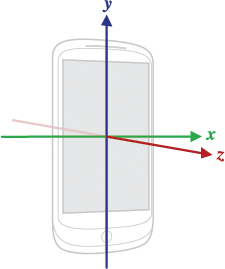
\includegraphics[width=5cm]{gambar/landasan-teori/axis_device.png}
    \caption{Sistem koordinat relatif terhadap perangkat yang digunakan dalam Android SDK (developer.android.com)}
    \label{gambar:koordinat-sensor-android}
\end{figure}

Sensor pada Android dapat diakses dengan membuat \mintinline{java}{SensorManager} yang diinisialisasi dengan \mintinline{java}{getSystemService(Context.SENSOR_SERVICE)}, seperti contoh berikut:

\begin{listing}[h]
    \begin{minted}{java}
        private SensorManager mSensorManager;
        private Sensor sensor;

        mSensorManager = (SensorManager)
        getSystemService(Context.SENSOR_SERVICE)
        sensor = mSensorManager.getDefaultSensor(JENIS_SENSOR)
    \end{minted}
\end{listing}


%------------------------------------------------------------------------------
% Akselerometer
%------------------------------------------------------------------------------
\section{Akselerometer}
Akselerometer adalah sensor yang digunakan untuk mengukur percepatan. Pada akselerometer \textit{Microelectrochemical System (MEMS)}, percepatan diukur dengan mengaitkan massa pada pegas dan melihat penyimpangan massa dari posisi setimbangnya \citep{milette-2012}, seperti yang diilustrasikan pada Gambar~\ref{gambar:akselerometer-mems}.

\begin{figure}[h!]
    \centering
    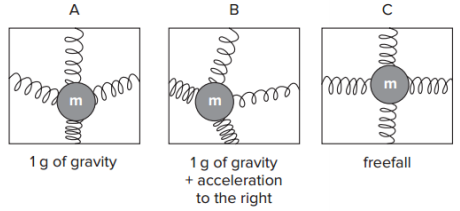
\includegraphics[width=10cm]{gambar/landasan-teori/akselerometer-mems.png}
    \caption{Gaya dikenakan pada massa yang terikat pada pegas \citep{milette-2012}}
    \label{gambar:akselerometer-mems}
\end{figure}

Pada sistem operasi Android, sensor akselerometer dapat diakses dengan menggunakan argumen \mintinline{java}{Sensor.TYPE_ACCELEROMETER} pada metode \mintinline{java}{getDefaultSensor()}, seperti contoh berikut:

\begin{listing}[h]
    \begin{minted}{java}
        private SensorManager mSensorManager;
        private Sensor accelerometer;

        mSensorManager = (SensorManager)
        getSystemService(Context.SENSOR_SERVICE)
        sensor = mSensorManager.getDefaultSensor(Sensor.TYPE_ACCELEROMETER)
    \end{minted}
\end{listing}

Data bacaan sensor disimpan dalam larik multidimensi pada \mintinline{java}{SensorEvent}. Data tersebut dapat dibaca dengan mengimplementasikan metode \textit{callback} \linebreak \mintinline{java}{onSensorChanged(SensorEvent event)}. Nilai bacaan sumbu x, y dan z akselerometer dapat diambil secara berurutan pada larik \mintinline{java}{SensorEvent.values} dengan indeks nol, satu dan dua. Berikut ini contoh pengambilan data sensor akselerometer:

\begin{listing}[h]
    \begin{minted}{java}
        public void onSensorChanged(SensorEvent event) {
            ax = event.values[0]
            ay = event.values[1]
            az = event.values[2]
        }
    \end{minted}
\end{listing}



%------------------------------------------------------------------------------
% Giroskop
%------------------------------------------------------------------------------
\section{Giroskop}
Seperti akselerometer MEMS, giroskop MEMS juga merupakan massa yang dikaitkan pada pegas. Giroskop MEMS digunakan untuk mengukur gaya coriolis yang terjadi karena rotasi. Giroskop MEMS bekerja dengan mendorong massa bolak-balik dalam satu sumbu. Ketika giroskop berputar, gaya coriolis membuat massa menyimpang dari arah getarannya sehingga bergerak ke arah sumbu yang berbeda. Pergerakan ini diukur secara elektrik dengan plat kapasitor, satu plat ditempatkan pada kerangka dan satu plat pada massa yang bergerak. Gaya coriolis hanya berlaku ketika perangkat berputar, sehingga giroskop dapat digunakan untuk mengukur kecepatan sudutnya \citep{milette-2012}.

Pada sistem operasi Android, sensor giroskop dapat diakses dengan menggunakan argumen \mintinline{java}{Sensor.TYPE_GYROSCOPE} pada metode \mintinline{java}{getDefaultSensor()}, seperti contoh berikut:

\begin{listing}[h]
    \begin{minted}{java}
        private SensorManager mSensorManager;
        private Sensor accelerometer;

        mSensorManager = (SensorManager)
        getSystemService(Context.SENSOR_SERVICE)
        sensor = mSensorManager.getDefaultSensor(Sensor.TYPE_GYROSCOPE)
    \end{minted}
\end{listing}

Seperti pada akselerometer, data bacaan sensor disimpan dalam larik multidimensi pada \mintinline{java}{SensorEvent}. Nilai bacaan sumbu x, y dan z giroskop dapat diambil secara berurutan pada larik \mintinline{java}{SensorEvent.values} dengan indeks nol, satu dan dua.


%------------------------------------------------------------------------------
% Pembelajaran Mesin
%------------------------------------------------------------------------------
\section{Pembelajaran Mesin}
Pembelajaran mesin adalah kemampuan komputer untuk beradaptasi dengan keadaan baru dan mendeteksi serta meramalkan kemungkinan pola. Terdapat tiga jenis \textit{feedback} yang menentukan tiga jenis utama pembelajaran mesin. \textit{Unsupervised learning} mempelajadi pola pada input meskiput tidak disediakan \textit{feedback} secara eksplisit, \textit{supervised learning} mengamati contoh pasangan input-output dan mempelajari fungsi yang memetakan dari input ke output, sedangkan \textit{reinforcement learning} melakukan pembelajaran dari rangkaian penghargaan atau hukuman \citep{Russell:2009:AIM:1671238}. Salah satu masalah yang berusaha diselesaikan proses pembelajaran mesin adalah klasifikasi, yaitu ketika output adalah satu dari himpunan terhingga nilai-nilai.


%------------------------------------------------------------------------------
% Deep Learning
%------------------------------------------------------------------------------
\section{Deep Learning}
Dalam pembelajaran mesin, performa suatu algoritma sangat bergantung pada representasi dari data yang digunakan. Setiap informasi yang menjadi representasi data disebut sebagai fitur.

Salah satu masalah dalam pembelajaran mesin adalah sulitnya mengetahui fitur-fitur apa saja yang harus diekstrak dari suatu set data. Masalah ini dapat diatasi dengan menggunakan pembelajaran mesin bukan hanya untuk menemukan pemetaan dari representasi ke output, tapi juga menemukan representasi itu sendiri. Pendekatan ini dikenal dengan \textit{representation learning} \citep{goodfellow-2016}.

Pada aplikasinya di dunia nyata, \textit{representation learning} sering mengalami kesulitan dalam menemukan representasi dari data yang kompleks. \textit{Deep learning} mengatasi masalah ini dengan membuat representasi yang disusun oleh representasi-representasi lain yang lebih sederhana.

\citeauthor{goodfellow-2016} mendefinisikan \textit{deep learning} sebagai salah satu jenis pembelajaran mesin yang memiliki kemampuan dan fleksibilitas tinggi dengan belajar merepresentasikan dunia sebagai hierarki konsep yang bersarang. Setiap konsep didefinisikan oleh kaitannya terhadap konsep-konsep yang lebih sederhana dan representasi yang lebih abstrak dihitung berdasarkan representasi yang kurang abstrak. Perbandingan \textit{deep learning} dengan sistem inteligensia buatan lainnya dapat dilihat pada Gambar~\ref{gambar:perbandingan-ai}.

\begin{figure}
    \centering
    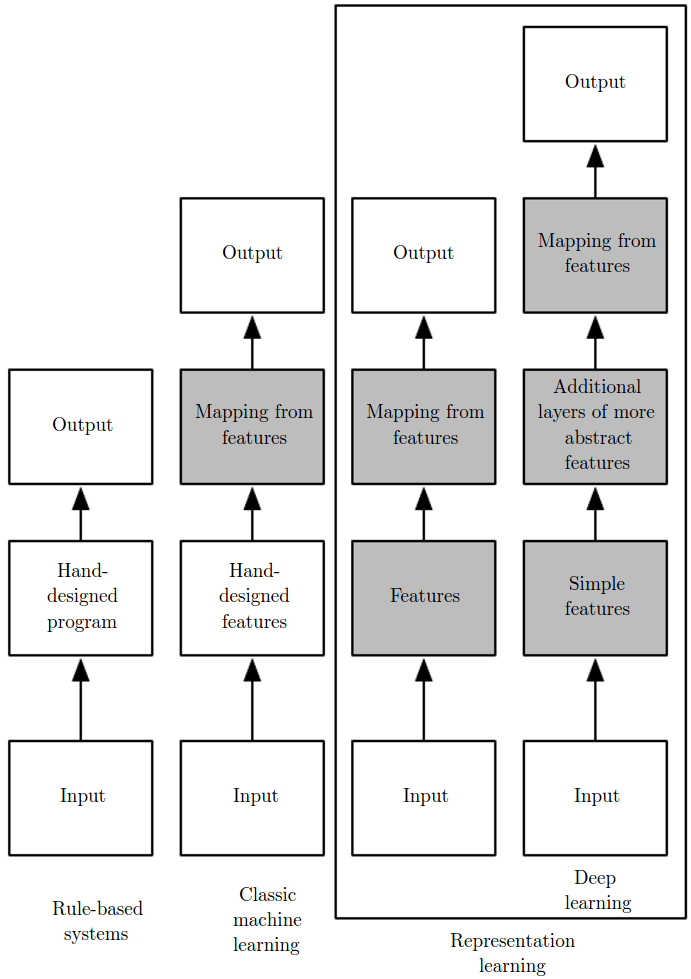
\includegraphics[width=12cm]{gambar/landasan-teori/perbandingan-ai.png}
    \caption{Perbandingan sistem AI. Kotak berwarna abu-abu menunjukkan komponen yang dapat belajar dari data \citep{goodfellow-2016}}
    \label{gambar:perbandingan-ai}
\end{figure}


%------------------------------------------------------------------------------
% Convolutional Neural Network
%
% TODO:
% - Apa perlu membahas sparse interactions, paramater sharing dan
%   equivariant representations?
% - Terjemahan paragraf pertama
%
%------------------------------------------------------------------------------
\section{Convolutional Neural Network}
Convolutional neural network (CNN) adalah jenis jaringan saraf untuk mengolah data \textit{grid-like topology}, seperti \textit{time-series data}, yang dapat dianggap sebagai grid 1D dengan sample pada interval tertentu, dan data citra, yang dapat dianggap sebagai 2D grid of pixels. CNN menggunakan operasi konvolusi untuk menggantikan operasi perkalian matriks pada setidaknya satu lapisan \citep{goodfellow-2016}. Operasi konvolusi dinotasikan sebagai:

\begin{equation}
    \label{eq:konvolusi}
    s(i) = (x * w)(i)
\end{equation}

Dalam terminologi CNN $x$ merupakan input, $w$ adalah kernel, dan outputnya disebut sebagai \textit{feature map}. Input $x$ merupakan larik multidimensi (tensor) parameter yang disesuaikan oleh algoritma pembelajaran.

Saat bekerja dengan data diskrit, persamaan~\ref{eq:konvolusi} dapat ditulis sebagai persamaan konvolusi diskrit:

\begin{equation}
    \label{eq:konvolusi-diskrit}
    s(i) = (x * w)(i) = \sum_{a=-\infty}^{\infty} x(a) w(i - a)
\end{equation}

Pada umumnya, konvolusi digunakan pada lebih dari satu sumbu. Misalnya, jika input adalah data dua dimensi seperti pada Gambar~\ref{gambar:konvolusi-2d}, maka digunakan kernel dua dimensi:
\begin{equation}
    \label{eq:konvolusi-2d}
    S(i,j) = (I * K)(i,j) = \sum_{m}\sum_{n}I(m,n)K(i-m, j-n)
\end{equation}

\begin{figure}[t!]
    \centering
    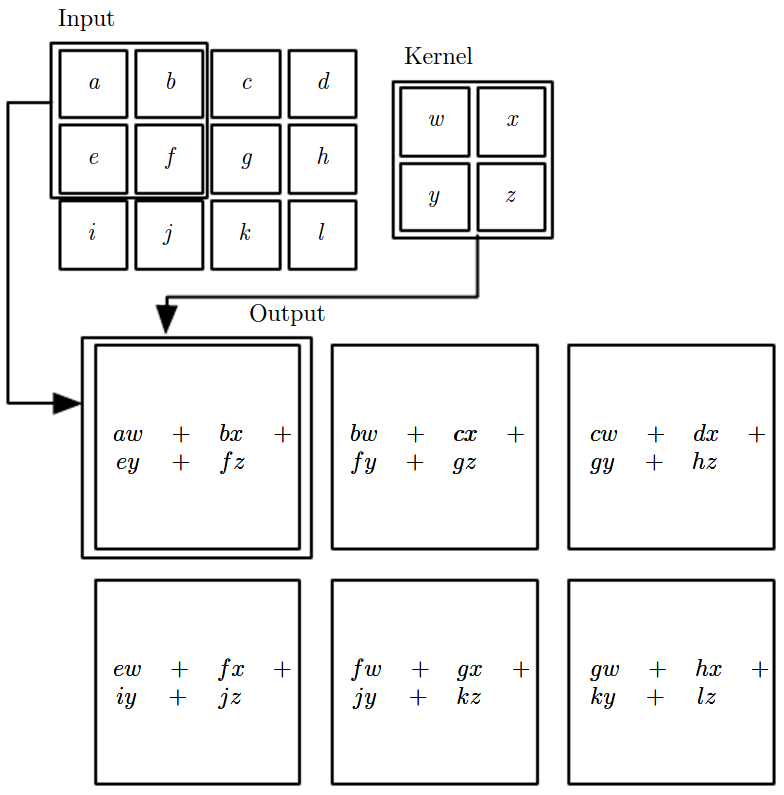
\includegraphics[width=10cm]{gambar/landasan-teori/konvolusi-2d.png}
    \caption{Contoh operasi konvolusi pada data dua dimensi \citep{goodfellow-2016}}
    \label{gambar:konvolusi-2d}
\end{figure}


%------------------------------------------------------------------------------
% Recurrent Neural Network
%
% TODO:
% - Ganti gambar RNN
%------------------------------------------------------------------------------
\section{Recurrent Neural Network}
Recurrent Neural Network (RNN) adalah keluarga jaringan saraf untuk memproses data sekuensial. RNN merupakan \textit{feedforward neural network} dengan hubungan yang berputar. Gambar~\ref{gambar:rnn} menunjukkan graf RNN dan graf yang setara namun telah dibentangkan berdasarkan langkah waktu. RNN dapat memetakan riwayat dari input sebelumnya ke setiap output. Dengan kata lain, koneksi yang berulang ini memungkinkan memori dari input sebelumnya tersimpan dalam kondisi internal jaringan, sehingga mempengaruhi output~\citep{graves-2012}.

\begin{figure}
    \centering
    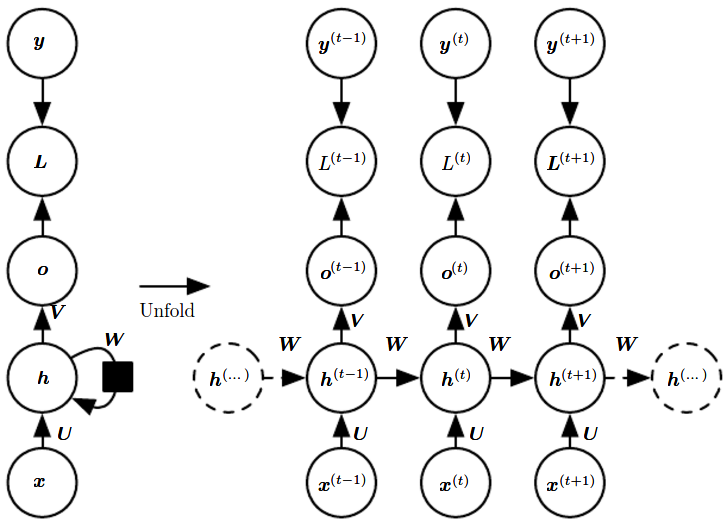
\includegraphics[width=10cm]{gambar/landasan-teori/rnn.png}
    \caption{Graf komputasi \textit{recurrent neural network} \citep{goodfellow-2016}}
    \label{gambar:rnn}
\end{figure}

Jika pada RNN dengan output diskrit diberikan output $\pmb{o}$ sebagai \textit{unormalized log probabilities} untuk setiap nilai yang mungkin dari variabel diskrit, operasi softmax dapat dilakukan sebagai langkah \textit{post-processing} untuk memperoleh vektor probabilitas normal $\pmb{\hat{y}}$ pada output. Propagasi maju dimulai dengan memberikan kondisi awal $\pmb{h}^{(0)}$. Lalu, pada setiap langkah waktu dari $t = 1$ sampai $t = \tau$, dilakukan perhitungan berikut:

\begin{align}
    \pmb{a}^{(t)} &= \pmb{b} + \pmb{Wh}^{(t-1)} + \pmb{Ux}^{(t)} \\
    \pmb{h}^{(t)} &= \tanh(\pmb{a}^{(t)}) \\
    \pmb{o}^{(t)} &= \pmb{c} + \pmb{Vh}^{(t)} \\
    \pmb{\hat{y}}^{(t)} &= softmax(\pmb{o}^{(t)})
\end{align}

\noindent
dengan $\pmb{b}$, $\pmb{c}$ vektor bias dan $\pmb{U}$, $\pmb{V}$, $\pmb{W}$ matriks bobot untuk hubungan input ke hidden, hidden ke output dan hidden ke hidden. Total \textit{loss} untuk pasangan $\pmb{x}$ dan $\pmb{y}$ dihitung dengan menjumlahkan \textit{loss} dari seluruh langkah waktu \citep{goodfellow-2016}.



%------------------------------------------------------------------------------
% Long Short-Term Memory
%------------------------------------------------------------------------------
\section{Long Short-Term Memory}
Long Short-Term Memory (LSTM) adalah salah satu jenis RNN bergerbang. Arsitektur LSTM terdiri dari kumpulan jaringan dengan hubungan internal berulang yang disebut dengan blok memori. Setiap blok memiliki satu atau lebih sel memori \textit{self-loop} dan tiga unit pengali, yaitu gerbang \textit{input, output} dan \textit{forget} \citep{graves-2012}.

\begin{figure}
    \centering
    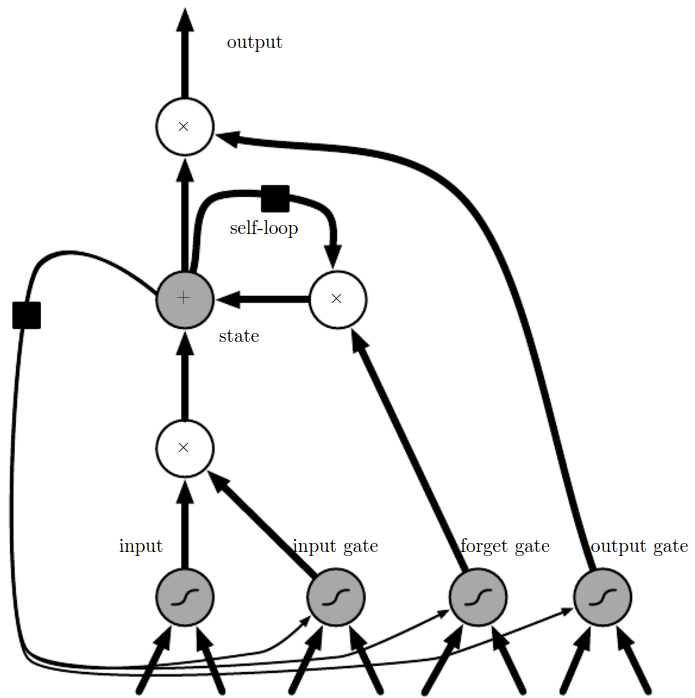
\includegraphics[width=10cm]{gambar/landasan-teori/lstm.png}
    \caption{Graf komputasi sel LSTM \citep{goodfellow-2016}}
    \label{gambar:lstm}
\end{figure}

Pada LSTM, bobot \textit{self-loop} dikendalikan oleh unit gerbang \textit{forget} $f_{i}^{(t)}$ (untuk langkah waktu $t$ dan sel $i$) yang memberikan nilai bobot antara 0 dan 1 melalui unit sigmoid:

\begin{equation}
    f_{i}^{(t)} = \sigma\left(b_{i}^{f} + \sum_{j} U_{i,j}^{f} x_{j}^{(t)} + \sum_{j} W_{i,j}^{f} h_{j}^{(t-1)}\right)
\end{equation}

\noindent
dengan $\pmb{x}^{(t)}$ vektor input saat ini, $\pmb{h}^{(t)}$ vektor \textit{hidden layer} saat ini yang berisi output dari seluruh sel LSTM, dan $\pmb{b}^{f}$, $\pmb{U}^{f}$, $\pmb{W}^{f}$ adalah bias, bobot input dan bobot pengulangan untuk gerbang \textit{forget}. Kondisi internal sel LSTM $s_{i}^{(t)}$ diperbarui sebagai berikut:

\begin{equation}
    s_{i}^{(t)} = f_{i}^{(t)}  s_{i}^{(t-1)} + g_{i}^{(t)} \sigma\left(b_{i} + \sum_{j} U_{i,j} x_{j}^{(t)} + \sum_{j} W_{i,j} h_{j}^{(t-1)} \right)
\end{equation}

\noindent
dengan $\pmb{b}, \pmb{U}$ dan $\pmb{W}$ sebagai bias, bobot input dan bobot pengulangan ke sel LSTM\@. Unit gerbang input eksternal $g_{i}^{(t)}$ dihitung dengan:

\begin{equation}
    g_{i}^{(t)} = \sigma\left(b_{i}^{g} + \sum_{j} U_{i,j}^{g} x_{j}^{(t)} + \sum_{j} W_{i,j}^{g} h_{j}^{(t-1)}\right)
\end{equation}

Output LSTM $h_{i}^{(t)}$ dapat dimatikan melalui gerbang output $q_{i}^{(t)}$, yang juga menggunakan unit sigmoid:

\begin{align}
    \label{eq:output-lstm}
    h_{i}^{(t)} &= \tanh\left(s_{i}^{(t)}\right) q_{i}{(t)} \\
    q_{i}^{(t)} &= \sigma\left(b_{i}^{o} + \sum_{j} U_{i,j}^{o} x_{j}^{(t)} + \sum_{j} W_{i,j}^{o} h_{j}^{(t-1)} \right)
\end{align}

\noindent
dengan $\pmb{b}^{o}, \pmb{U}^{o}$ dan $\pmb{W}^{o}$ sebagai bias, bobot input dan bobot pengulangan \citep{goodfellow-2016}.

% \section{Stochastic Gradient Descent}


%------------------------------------------------------------------------------
% Backpropagation Through Time
%------------------------------------------------------------------------------
\section{Backpropagation Through Time}
Kebanyakan algoritma \textit{deep learning} membutuhkan proses optimasi, yaitu proses meminimalkan atau memaksimalkan suatu fungsi $f(\pmb{x})$ dengan mengubah $\pmb{x}$. Fungsi yang akan diminimalkan atau dimaksimalkan disebut fungsi objektif. Dalam kasus meminimalkan, fungsi objektif bisa juga disebut \textit{cost function}, \textit{loss function} atau \textit{error function} \citep{goodfellow-2016}.

\citeauthor{goodfellow-2016} menambahkan, jika diberikan fungsi $y = f(x)$ dengan $x$ dan $y$ bilangan real, derivatif dari fungsi ini adalah gradien $f(x)$ pada titik $x$, dinotasikan dengan $f'(x)$ atau $\frac{dy}{dx}$. Fungsi $f(x)$ dapat diminimalkan dengan membuat perubahan $x$ ke arah yang berlawanan dengan derivatifnya. Cara ini disebut \textit{gradient descent}, diilustrasikan pada Gambar~\ref{gambar:gradient-descent}.

\begin{figure}
    \centering
    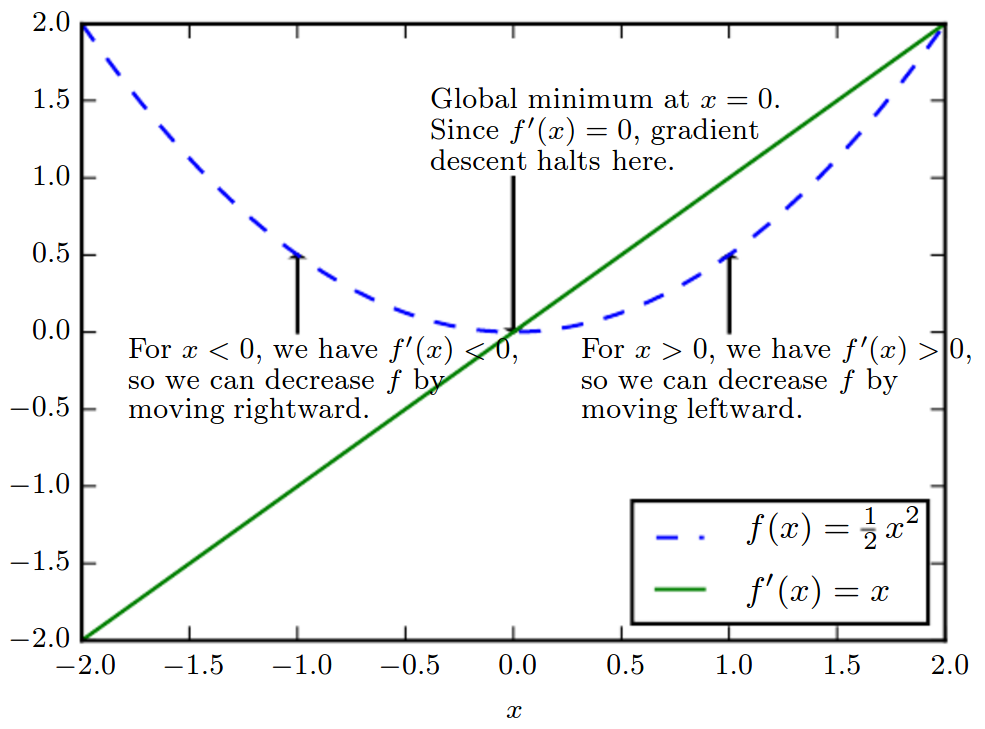
\includegraphics[width=12cm]{gambar/landasan-teori/gradient-descent.png}
    \caption{\textit{Gradient descent} menggunakan derivatif untuk meminimalkan sebuah fungsi \citep{goodfellow-2016}}.
    \label{gambar:gradient-descent}
\end{figure}

Ketika \textit{feedforward neural network} menerima input $\pmb{x}$ dan menghasilkan output $\pmb{\hat{y}}$, informasi mengalir maju melalui jaringan. Input $\pmb{x}$ menyediakan informasi awal yang merambat ke \textit{hidden unit} pada setiap layer hingga akhirnya menghasilkan $\pmb{\hat{y}}$. Proses ini disebut \textit{forward propagation}. Dalam proses latihan, \textit{forward propagation} dapat terus maju sampai menghasilkan nilai skalar \textit{cost} $J(\theta)$. Algoritma \textit{backpropagation} memungkinkan informasi dari \textit{cost} mengalir mundur melalui jaringan untuk menghitung gradiennya \citep{goodfellow-2016}.

\textit{Backpropagation} menghitung derivatif fungsi dengan aturan rantai kalkulus. \citet{nielsen-2015} mendefinisikan algoritma backpropagation dalam lima langkah:
\begin{enumerate}
    \item Input x: Atur aktivasi $a^{l}$ untuk lapisan input
    \item Feedforward: Untuk setiap $l = 2, 3, \ldots, L$ hitung $z^{l} = w^{l} a^{l-1} + b^{l}$ dan $a^{l} = \sigma (z^{l})$
    \item Output error $\delta^{L}$: Hitung vektor $\delta^{L} = \nabla_{a} C \odot \sigma ' (z^{L})$
    \item Rambatkan error ke belakang: Untuk setiap $l = L-1, L-2, \ldots, 2$ hitung $\delta^{l} = ({(w^{l+1})}^{T} \delta^{l+1}) \odot \sigma' (z^{l})$
    \item Output: Hitung gradient dari \textit{cost function} dengan $\frac{\partial C}{\partial w_{jk}^{l}} = a_{k}^{l-1} \delta_{j}^{l}$ dan $\frac{\partial C}{\partial b_{j}^{l}} = \delta_{j}^{l}$
\end{enumerate}

\noindent
dengan $L$ jumlah lapisan dalam jaringan, $C$ \textit{cost function}, $w_{jk}^{l}$ bobot koneksi dari neuron ke-$k$ pada lapisan $(l-1)$ ke neuron ke-$j$ pada lapisan $l$ dan $b_{j}^{l}$ bias neuron ke-$j$ pada lapisan $l$.

Pada RNN, aktivasi \textit{hidden layer} tidak hanya mempengaruhi \textit{loss function} pada \textit{output layer}, namun juga mempengaruhi \textit{hidden layer} pada langkah waktu selanjutnya. Maka, gradien dihitung dengan menggunakan \textit{backpropagation} pada graf yang telah dibentangkan. Metode ini bernama \textit{backpropagation through time (BPTT)} \citep{graves-2012}.


%------------------------------------------------------------------------------
% Tensorflow
%------------------------------------------------------------------------------
\section{TensorFlow}
TensorFlow adalah pustaka sumber terbuka pembalajaran mesin. TensorFlow melakukan komputasi yang dideskripsikan dengan model aliran data dan memetakannya ke berbagai jenis perangkat keras berbeda, mulai dari melakukan pengambilan kesimpulan pada perangkat bergerak seperti Android dan iOS, pelatihan dan sistem pengambilan keputusan berukuran sedang menggunakan satu mesin yang terdiri dari satu atau lebih kartu GPU sampai ke sistem pelatihan berskala besar yang berjalan pada ratusan mesin khusus dengan ribuan GPU \citep{abadi-2015}.

\begin{figure}
    \centering
    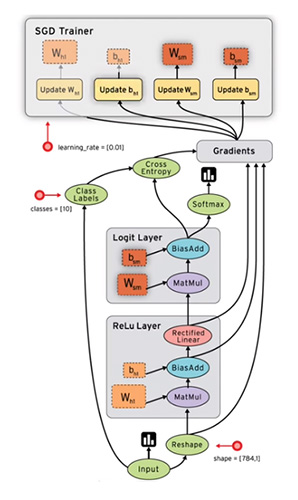
\includegraphics[width=6cm]{gambar/landasan-teori/tensorflow.jpg}
    \caption{Contoh graf aliran data dalam TensorFlow (tensorflow.com)}
    \label{gambar:tensorflow}
\end{figure}

Graf aliran data dalam TensorFlow mendeskripsikan komputasi matematis dengan graf \textit{node} dan \textit{edge} terarah. \textit{Edge} memuat array multidimensi berukuran dinamis yang disebut dengan tensor. Para \textit{node} bekerja secara asinkron dan paralel ketika seluruh tensor pada \textit{edge} yang masuk telah tersedia. Contoh graf aliran data pada TensorFlow dapat dilihat pada Gambar~\ref{gambar:tensorflow}. Aliran data tersebut direpresentasikan oleh TensorFlow melalui API yang tersedia untuk bahasa Python, C++, Java dan Go.



\chapter{ANALISIS DAN PERANCANGAN SISTEM}


%------------------------------------------------------------------------------
% Analisis Sistem
%------------------------------------------------------------------------------
\section{Analisis Sistem}
Pada penelitian ini dibuat sistem untuk mengenali aktivitas manusia secara \textit{real time} dengan sensor akselerometer dan giroskop yang tertanam pada ponsel cerdas. Rancangan sistem ini dapat dilihat pada Gambar~\ref{gambar:diagram-blok-sistem}.

\begin{figure}[h!]
    \centering
    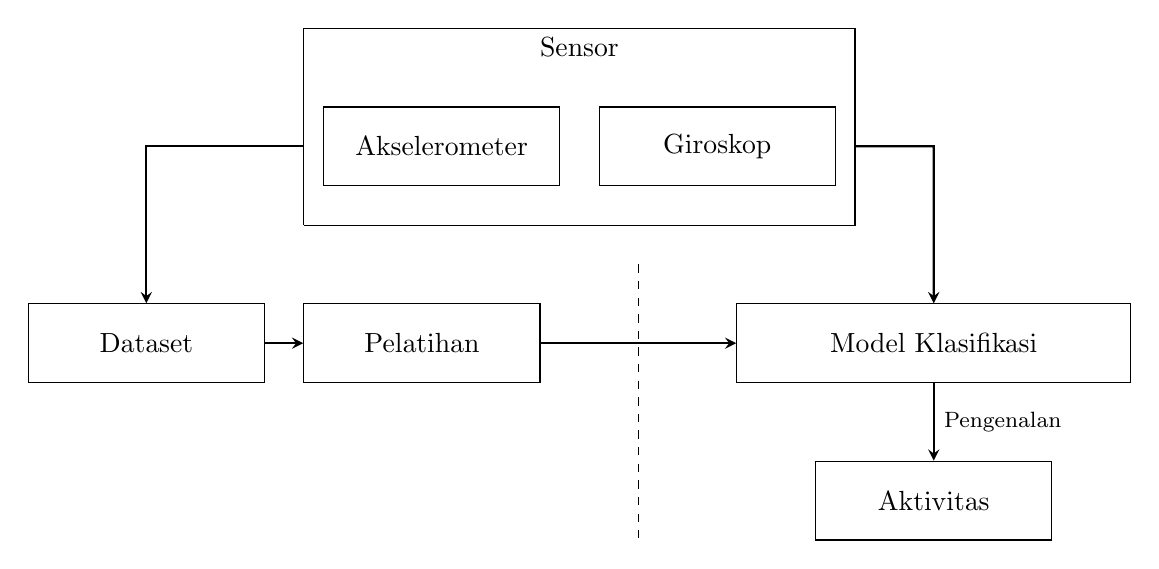
\begin{tikzpicture}[node distance=1.5cm]
        \node (dataset) [process] {Dataset};
        \node (pelatihan) [process, right of=dataset, xshift=2cm] {Pelatihan};
        \node (model-klasifikasi) [process, right of=pelatihan, xshift=5cm, minimum width=5cm] {Model Klasifikasi};  
        \node (akselerometer) [process, above of=model-klasifikasi, xshift=-6.25cm, yshift=1cm] {Akselerometer};
        \node (giroskop) [process, right of=akselerometer, xshift=2cm] {Giroskop};
        \draw (2,1.5) -- (9,1.5) -- (9,4) -- node[anchor=north] {Sensor} (2,4) -- (2,1.5);
        \node (aktivitas) [process, below of=model-klasifikasi, yshift=-0.5cm] {Aktivitas};

        \draw [arrow] (dataset) -- (pelatihan);
        \draw [arrow] (pelatihan) -- (model-klasifikasi);
        \draw [arrow] (9,2.5) -- (10,2.5) -- (model-klasifikasi);
        \draw [arrow] (2,2.5) -- (0,2.5) -- (dataset);
        \draw [arrow] (model-klasifikasi) -- node[anchor=west, font=\footnotesize] {Pengenalan} (aktivitas);
        \draw [dashed] (6.25, 1) -- (6.25, -2.5);
    \end{tikzpicture}
    \caption{Diagram blok sistem}
    \label{gambar:diagram-blok-sistem}
\end{figure}

Sistem ini memanfaatkan model klasifikasi yang disusun dari lapisan-lapisan \textit{Convolutional Neural Network} (CNN) dan \textit{Long Short-Term Memory} (LSTM) untuk mengklasifikasikan bacaan sensor akselerometer dan giroskop menjadi enam aktivitas sederhana, yaitu duduk, berdiri, berjalan, berlari, menaiki tangga dan menuruni tangga.

Sebelum dapat melakukan klasifikasi, model dilatih dengan dataset aktivitas manusia. Dalam proses pelatihan tersebut, model klasifikasi menerima masukan dari data latih lalu mengoptimasi parameter-parameternya untuk menghasilkan klasifikasi yang lebih baik. Setelah dilatih, model diimplementasikan pada ponsel cerdas Android untuk melakukan pengenalan aktivitas manusia secara \textit{real time} dari data sensor akselerometer dan giroskop yang tertanam.

%------------------------------------------------------------------------------
% Peralatan
%------------------------------------------------------------------------------
\section{Peralatan}
Peralatan yang digunakan untuk mendukung penelitian ini terdiri dari perangkat keras dan perangkat lunak berikut:

\subsection{Perangkat Keras}
\begin{enumerate}
    \item Laptop HP 14--015tx dengan CPU Intel Core i5--6200U 2.3 GHz dan RAM 12GB
    \item Ponsel cerdas Android dengan sensor akselerometer dan giroskop tertanam
\end{enumerate}

\subsection{Sistem Perangkat Lunak}
\begin{enumerate}
    \item Ubuntu 16.04 64 bit sebagai sistem operasi laptop
    \item TensorFlow sebagai pustaka komputasi numerik
    \item Visual Studio Code sebagai \textit{text editor} untuk menulis program sistem klasifikasi
    \item Android Studio sebagai \textit{Integrated Development Environment} (IDE) untuk mengembangkan aplikasi Android
\end{enumerate}

%------------------------------------------------------------------------------
% Rancangan Perangkat Lunak
%------------------------------------------------------------------------------
\subsection{Rancangan Perangkat Lunak}
Sistem dirancang untuk mengklasifikasikan aktivitas manusia berdasarkan data dari sensor akselerometer dan giroskop pada ponsel cerdas. Aliran data sensor pada proses klasifikasi dan pelatihan ditunjukkan pada Gambar~\ref{gambar:aliran-data-klasifikasi}. Diagram tersebut menggambarkan graf komputasi model klasifikasi serta proses pelatihan yang dilakukan untuk mengoptimasi parameter-paramter pada model.

\begin{figure}[h!]
    \centering
    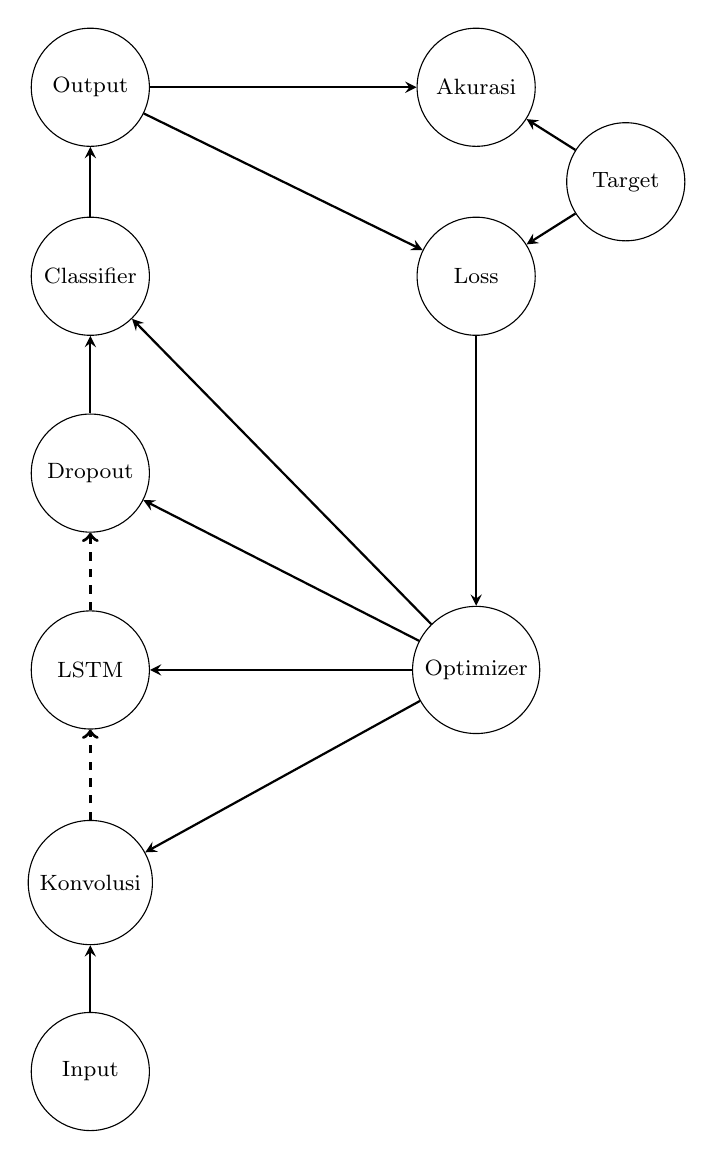
\begin{tikzpicture}[node distance=1.9cm]
        \node (input) [state] {Input};
        \node (cnn) [state, above of=input, yshift=0.5cm] {Konvolusi};
        \node (lstm) [state, above of=cnn, yshift=0.8cm] {LSTM};
        \node (dropout) [state, above of=lstm, yshift=0.6cm] {Dropout};
        \node (softmax) [state, above of=dropout, yshift=0.6cm] {Classifier};
        \node (output) [state, above of=softmax, yshift=0.5cm] {Output};
        \node (loss) [state, right of=softmax, xshift=3cm] {Loss};
        \node (akurasi) [state, right of=output, , xshift=3cm] {Akurasi};
        \node (target) [state, right of=loss, yshift=1.2cm] {Target};
        \node (optimizer) [state, right of=lstm, xshift=3cm] {Optimizer};

        \draw [arrow] (input) -- (cnn);
        \draw [dashed, very thick,->] (cnn) -- (lstm);
        \draw [dashed, very thick,->] (lstm) -- (dropout);
        \draw [arrow] (dropout) -- (softmax);
        \draw [arrow] (softmax) -- (output);
        \draw [arrow] (output) -- (loss);
        \draw [arrow] (output) -- (akurasi);
        \draw [arrow] (target) -- (loss);
        \draw [arrow] (target) -- (akurasi);
        \draw [arrow] (loss) -- (optimizer);
        \draw [arrow] (optimizer) -- (cnn);
        \draw [arrow] (optimizer) -- (lstm);
        \draw [arrow] (optimizer) -- (dropout);
        \draw [arrow] (optimizer) -- (softmax);
    \end{tikzpicture}
    \caption{Aliran data pada proses klasifikasi dan pelatihan}
    \label{gambar:aliran-data-klasifikasi}
\end{figure}

\section{Model Klasifikasi}

Proses klasifikasi dilakukan dalam beberapa langkah. Pertama, pra pengolahan dilakukan pada data masukan untuk pengondisian. Data tersebut kemudian dimasukkan ke dalam beberapa lapisan konvolusi. Setelah itu hasil lapisan konvolusi dimasukkan ke dalam beberapa lapisan LSTM\@. Kedua lapisan ini menghasilkan fitur-fitur abstrak yang merepresentasikan data sensor. Fitur-fitur ini kemudian diklasifikasikan dalam lapisan \textit{classifier}. Lapisan ini menggunakan fungsi \textit{softmax} yang menghasilkan distribusi peluang kelas aktivitas dari data masukan. Hubungan antara lapisan LSTM dan lapisan \textit{classifier} diregulasi dengan \textit{dropout} untuk mengurangi \textit{overfitting}.

\subsection{Data Masukan}
Data masukan adalah rangkaian data \textit{time series} dari sensor akselerometer dan giroskop. Rangkaian data tersebut diambil dari ponsel cerdas dan dikelompokkan menggunakan \textit{sliding window} pada setiap 100 langkah waktu dengan \textit{overlap} 50\%.

Sensor akselerometer dan giroskop menghasilkan nilai bacaan dengan tiga sumbu, yaitu sumbu $x$, $y$ dan $z$. Nilai sensor akselerometer $\pmb{a}$ dan giroskop $\pmb{g}$ dinotasikan sebagai vektor~\ref{eq:vektor-akselerometer} dan~\ref{eq:vektor-giroskop}.

\begin{equation}
    \label{eq:vektor-akselerometer}
    \pmb{a} = 
    \begin{bmatrix}
        a_x \\
        a_y \\
        a_z
    \end{bmatrix}
\end{equation}

\begin{equation}
    \label{eq:vektor-giroskop}
    \pmb{g} = 
    \begin{bmatrix}
        g_x \\
        g_y \\
        g_z
    \end{bmatrix}
\end{equation}

Nilai sensor pada sumbu $x$, $y$ dan $z$ dipengaruhi oleh posisi dan arah gerak sensor. Mengingat posisi ponsel cerdas saat digunakan tidak menentu, maka perlu dicari nilai yang tidak dipengaruhi oleh arah gerak sensor, yaitu besar dari masing-masing vektor $\pmb{a}$ dan $\pmb{g}$. Besar vektor akseleromter dan giroskop dapat dicari dengan Persamaan~\ref{eq:norm-akselerometer} dan~\ref{eq:norm-giroskop}.

\begin{equation}
    \label{eq:norm-akselerometer}
    |\pmb{a}| = \sqrt{a_x^2 + a_y^2 + a_z^2}
\end{equation}

\begin{equation}
    \label{eq:norm-giroskop}
    |\pmb{g}| = \sqrt{g_x^2 + g_y^2 + g_z^2}
\end{equation}

Model klasifikasi menerima masukan matriks $\pmb{X}_{t \times n}$ dengan ukuran $t = 100$ dan $n = 8$. Setiap baris tersebut merupakan \textit{sample} sensor akselerometer dan giroskop dalam satu langkah waktu yang diurutkan dari waktu $t_1$ sampai $t_{100}$. Matriks $\pmb{X}$ ditunjukkan dalam Persamaan~\ref{eq:matriks-masukan}.

\begin{equation}
    \label{eq:matriks-masukan}
    \pmb{X}_{t \times n} =
    \begin{bmatrix}
        a_x^{(0)} & a_y^{(0)} & a_z^{(0)} & |\pmb{a}|^{(0)} & g_x^{(0)} & g_y^{(0)} & g_z^{(0)} & |\pmb{g}|^{(0)} \\
        a_x^{(1)} & a_y^{(1)} & a_z^{(1)} & |\pmb{a}|^{(1)} & g_x^{(1)} & g_y^{(1)} & g_z^{(1)} & |\pmb{g}|^{(1)} \\
        \cdots & \cdots & \cdots & \cdots & \cdots & \cdots & \cdots & \cdots \\
        a_x^{(100)} & a_y^{(100)} & a_z^{(100)} & |\pmb{a}|^{(100)} & g_x^{(100)} & g_y^{(100)} & g_z^{(100)} & |\pmb{g}|^{(100)} \\
        
    \end{bmatrix}
\end{equation}

\subsection{Lapisan Konvolusi}
Diagram blok lapisan konvolusi ditunjukkan pada Gambar~\ref{gambar:diagram-blok-kovolusi}. Matriks masukan $\pmb{X}$ dilewatkan melalui lapisan kovolusi untuk mencari fitur-fitur dari data sensor. Lapisan konvolusi menggunakan kernel $\pmb{K}_{m \times n}$, masing-masing nilai anggotanya adalah bobot yang digunakan bersama oleh setiap jendela komputasi. Jumlah lapisan konvolusi dan ukuran kernel $m \times n$ merupakan \textit{hyperparameter} yang diatur sebelum pelatihan.

\begin{figure}[h!]
    \centering
    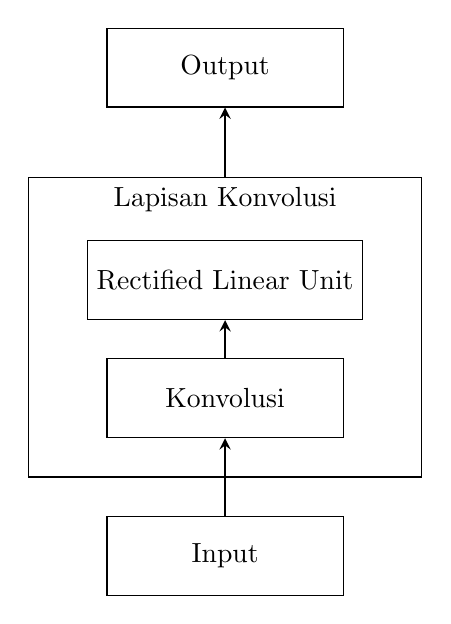
\begin{tikzpicture}[node distance=1.5cm]
        \node (input) [process] {Input};
        \node (konvolusi) [process, above of=input, yshift=0.5cm] {Konvolusi};
        \node (relu) [process, above of=konvolusi] {Rectified Linear Unit};
        \node (output) [process, above of=relu, yshift=1.2cm] {Output};
        \draw (-2.5,4.8) -- node[anchor=north] {Lapisan Konvolusi} (2.5,4.8) -- (2.5,1) -- (-2.5,1) -- (-2.5,4.8);

        \draw [arrow] (input) -- (konvolusi);
        \draw [arrow] (konvolusi) -- (relu);
        \draw [arrow] (0,4.8) -- (output);
    \end{tikzpicture}
    \caption{Diagram blok lapisan konvolusi}
    \label{gambar:diagram-blok-kovolusi}
\end{figure}

Nilai keluaran lapisan konvolusi dapat dihitung dengan melakukan konvolusi antara jendela komputasi $\pmb{I}$ dengan bobot $\pmb{W}$. Hasil konvolusi ditambahkan dengan bias dan dimasukkan ke dalam fungsi aktivasi \textit{Rectified Linear Unit} (ReLU)\@. Operasi tersebut didefinisikan sebagai

\begin{equation}
    H(i,j) = g((\pmb{I} * \pmb{W})(i,j) + \pmb{b})
    \label{eq:konvolusi-kernel}
\end{equation}

\noindent
dengan

\begin{equation}
    (\pmb{I} * \pmb{W})(i,j) = \sum_{m}\sum_{n}I(m,n)W(i-m, j-n)
    \label{eq:konvolusi-3d}
\end{equation}

\noindent
dan fungsi aktivasi ReLU didefinisikan dalam persamaan

\begin{equation}
    g(z) = \max(0,z)
    \label{eq:relu}
\end{equation}

Perhitungan dilakukan untuk setiap jendela komputasi. Berikut ini tahapan perhitungan dalam lapisan konvolusi:

\begin{enumerate}
\item Jendela komputasi $\pmb{I}$ dibuat dari $\pmb{X}$ dengan ukuran $m \times n$
\item Untuk setiap jendela, lakukan perhitungan konvolusi dengan Persamaan~\ref{eq:konvolusi-kernel}.
\item Lakukan tahap 1 dan 2 dengan langkah antar jendela 1
\item Susun hasil perhitungan setiap jendela menjadi matriks $\pmb{H}$
\end{enumerate}

\subsection{Lapisan LSTM}
Output dari lapisan konvolusi dilewatkan melalui lapisan LSTM\@. Jumlah lapisan LSTM $L$ dan jumlah \textit{hidden unit} pada masing-masing lapisan merupakan \textit{hyperparameter} yang ditentukan sebelum pelatihan. Setiap lapisan memiliki bobot antar input ke hidden $\pmb{U}$, bobot antar hidden ke output $\pmb{V}$, bobot antar hidden ke hidden $\pmb{W}$, serta bias $\pmb{b}$ dan $\pmb{c}$. Jika diberikan input matriks $\pmb{X}_{m \times n}$, $\pmb{x}^{(t)}$ merupakan subset dari $\pmb{X}$ pada langkah waktu $t$ dari $t = 1$ sampai $t = m$. Keluaran LSTM $\pmb{h}^{(t)}$ dapat dicari dengan Persamaan~\ref{eq:output-lstm}.

\begin{figure}[h!]
    \centering
    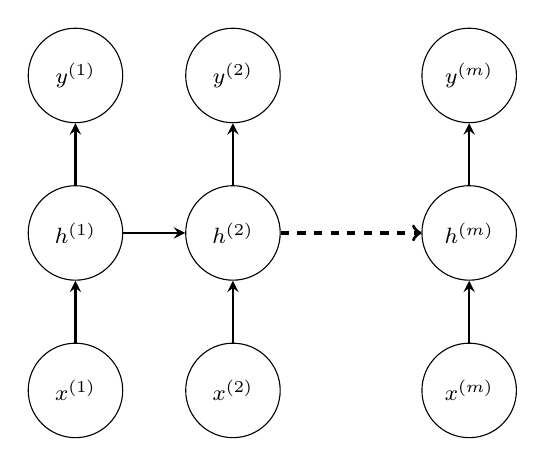
\begin{tikzpicture}[node distance=2cm]
        \node (x1) [cell] {$x^{(1)}$};
        \node (x2) [cell, right of=x1] {$x^{(2)}$};
        \node (xm) [cell, right of=x2, xshift=1cm] {$x^{(m)}$};
        \node (h1) [cell, above of=x1] {$h^{(1)}$};
        \node (h2) [cell, above of=x2] {$h^{(2)}$};
        \node (hm) [cell, above of=xm] {$h^{(m)}$};
        \node (y1) [cell, above of=h1] {$y^{(1)}$};
        \node (y2) [cell, above of=h2] {$y^{(2)}$};
        \node (ym) [cell, above of=hm] {$y^{(m)}$};

        \draw [arrow] (x1) -- (h1);
        \draw [arrow] (x2) -- (h2);
        \draw [arrow] (xm) -- (hm);
        \draw [arrow] (h1) -- (y1);
        \draw [arrow] (h2) -- (y2);
        \draw [arrow] (hm) -- (ym);
        \draw [arrow] (h1) -- (h2);
        \draw [dashed, very thick,->] (h2) -- (hm);
    \end{tikzpicture}
    \caption{Arsitektur lapisan LSTM \textit{many-to-many}}
    \label{gambar:many-to-many}
\end{figure}

\begin{figure}[h!]
    \centering
    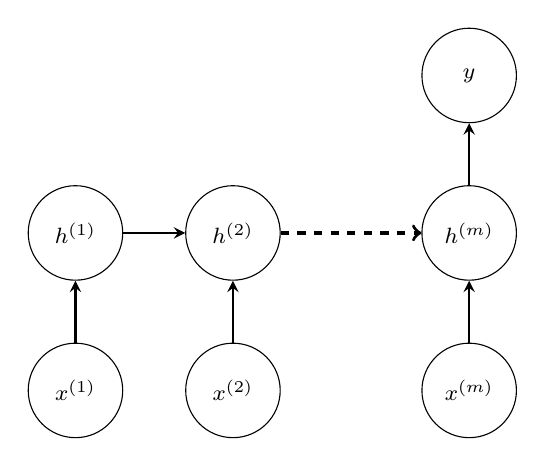
\begin{tikzpicture}[node distance=2cm]
        \node (x1) [cell] {$x^{(1)}$};
        \node (x2) [cell, right of=x1] {$x^{(2)}$};
        \node (xm) [cell, right of=x2, xshift=1cm] {$x^{(m)}$};
        \node (h1) [cell, above of=x1] {$h^{(1)}$};
        \node (h2) [cell, above of=x2] {$h^{(2)}$};
        \node (hm) [cell, above of=xm] {$h^{(m)}$};
        \node (y) [cell, above of=hm] {$y$};

        \draw [arrow] (x1) -- (h1);
        \draw [arrow] (x2) -- (h2);
        \draw [arrow] (xm) -- (hm);
        \draw [arrow] (hm) -- (y);
        \draw [arrow] (h1) -- (h2);
        \draw [dashed, very thick,->] (h2) -- (hm);
    \end{tikzpicture}
    \caption{Arsitektur lapisan LSTM \textit{many-to-one}}
    \label{gambar:many-to-one}
\end{figure}

Sel-sel LSTM pada lapisan pertama sampai lapisan ke $L-1$ disusun dengan arsitektur \textit{many-to-many} seperti pada Gambar~\ref{gambar:many-to-many}, sedangkan sel-sel LSTM pada lapisan ke-$L$ disusun dengan arsitektur \textit{many-to-one} seperti pada Gambar~\ref{gambar:many-to-one}. Input lapisan LSTM pertama diambil dari output lapisan konvolusi, sedangkan input lapisan LSTM selanjutnya diambil dari output lapisan LSTM sebelumnya. Output dari lapisan LSTM terakhir hanya diambil dari keluaran pada langkah waktu terakhir, yaitu $\pmb{h}^{(t)}$ pada saat $t = m$.

\subsection{\textit{Classifier}}
Output dari lapisan LSTM masuk ke lapisan \textit{classifier} dan diregulasi dengan \textit{dropout} untuk mencegah \textit{overfitting}. Lapisan \textit{classifier} adalah jaringan padat yang menggunakan fungsi \textit{softmax} sebagai fungsi aktivasinya. Fungsi aktivasi \textit{softmax} digunakan untuk mencari distribusi peluang seluruh kelas aktivitas manusia.

Jaringan padat adalah jaringan dengan neuron yang seluruhnya terhubung dengan neuron pada lapisan sebelum atau sesudahnya. Jaringan padat dengan enam neuron dibuat dengan masukan dari hasil lapisan LSTM terakhir. Jumlah neuron tersebut dipilih sesuai dengan jumlah aktivitas yang akan diklasifikasikan.

Lapisan \textit{classifier} menerima masukan vektor $\pmb{x}$. Dengan bobot $\pmb{W}$ dan bias $\pmb{b}$, keluaran lapisan ini dihitung menggunakan persamaan

\begin{equation}
    \pmb{y} = softmax(\pmb{W} \pmb{x} + \pmb{b})
\end{equation}

\noindent
dan fungsi \textit{softmax} didefinisikan sebagai

\begin{equation}
    softmax(\pmb{z})_i = \frac{\exp(z_i)}{\sum_{j=1}^n \exp(z_j)}
\end{equation}

Persamaan di atas menghasilkan vektor distribusi peluang dari enam kelas aktivitas. Aktivitas yang dikenali adalah aktivitas dengan peluang tertinggi.

\section{Dataset Aktivitas Manusia}
Model klasifikasi dilatih dengan dataset yang dikumpulkan dari 48 parisipan (36 laki-laki dan 12 perempuan) dalam rentang usia antara 20 sampai 28 tahun. Setiap partisipan melakukan aktivitas duduk, berdiri, berjalan, berlari, menaiki tangga dan menuruni tangga dengan menempatkan ponsel cerdas di saku celana. Data sensor akselerometer dan giroskop diambil dengan \textit{sampling rate} 50 Hz, lalu \textit{sliding window} dibuat dari setiap 100 sample dengan \textit{overlap} 50\%. Dengan aturan tersebut, diperoleh data aktivitas seperti pada Tabel~\ref{table:jumlah-dataset}.

\begin{table}[h!]
    \centering
    \caption{Jumlah dataset}
    \begin{tabular}{ |l|c| }
        \hline
        Aktivitas & Jumlah Sampel \\

        \hline
        Berdiri & 14.394 \\

        \hline
        Duduk & 1.710 \\

        \hline
        Berjalan & 14.394 \\

        \hline
        Berlari & 4.314 \\

        \hline
        Menaiki Tangga & 2.844 \\

        \hline
        Menuruni Tangga & 2.864 \\

        \hline
        Total & 40.520 \\

        \hline
    \end{tabular}
    \label{table:jumlah-dataset}
\end{table}

Proses pelatihan membutuhkan tiga jenis data, yaitu data latih, data validasi dan data uji. Data latih digunakan untuk melatih model dalam optimasi parameter yang menghasilkan klasifikasi terbaik, data validasi digunakan untuk mengukur kemampuan model seiring berjalannya proses palatihan, sedangkan data uji digunakan untuk mengukur kemampuan model akhir hasil pelatihan. Data latih, data validasi dan data uji diambil dari partisipan yang berbeda. Pembagian data tersebut dapat dilihat pada Tabel~\ref{table:pembagian-data}.

\begin{table}[h!]
    \centering
    \caption{Pembagian data latih, validasi dan uji}
    \begin{tabular}{ |l|c|c| }
        \hline
        Jenis Data & Partisipan & Jumlah Sampel \\

        \hline
        Data Latih & 27 & 22.776 \\

        \hline
        Data Validasi & 7 & 5.928 \\

        \hline
        Data Uji & 14 & 11.816 \\

        \hline
        Total & 48 & 40.520 \\

        \hline
    \end{tabular}
    \label{table:pembagian-data}
\end{table}

\section{Pelatihan}
Proses pelatihan jaringan dilakukan untuk mencari bobot dan bias yang optimal pada seluruh neuron dalam setiap lapisan. Optimasi bobot dan bias tersebut dilakukan dengan meminimal \textit{cost function} dengan proses \textit{backpropagation}. Diagram alir proses pelatihan ditunjukkan pada gambar~\ref{gambar:diagram-alir-pelatihan}. Model klasifikasi disusun sebagai graf yang sesuai dengan masukan \textit{hyperparameter}. Kemudian model ini dilatih dalam sebuah iterasi.

\begin{figure}[h]
    \centering
    \scalebox{0.8}{
        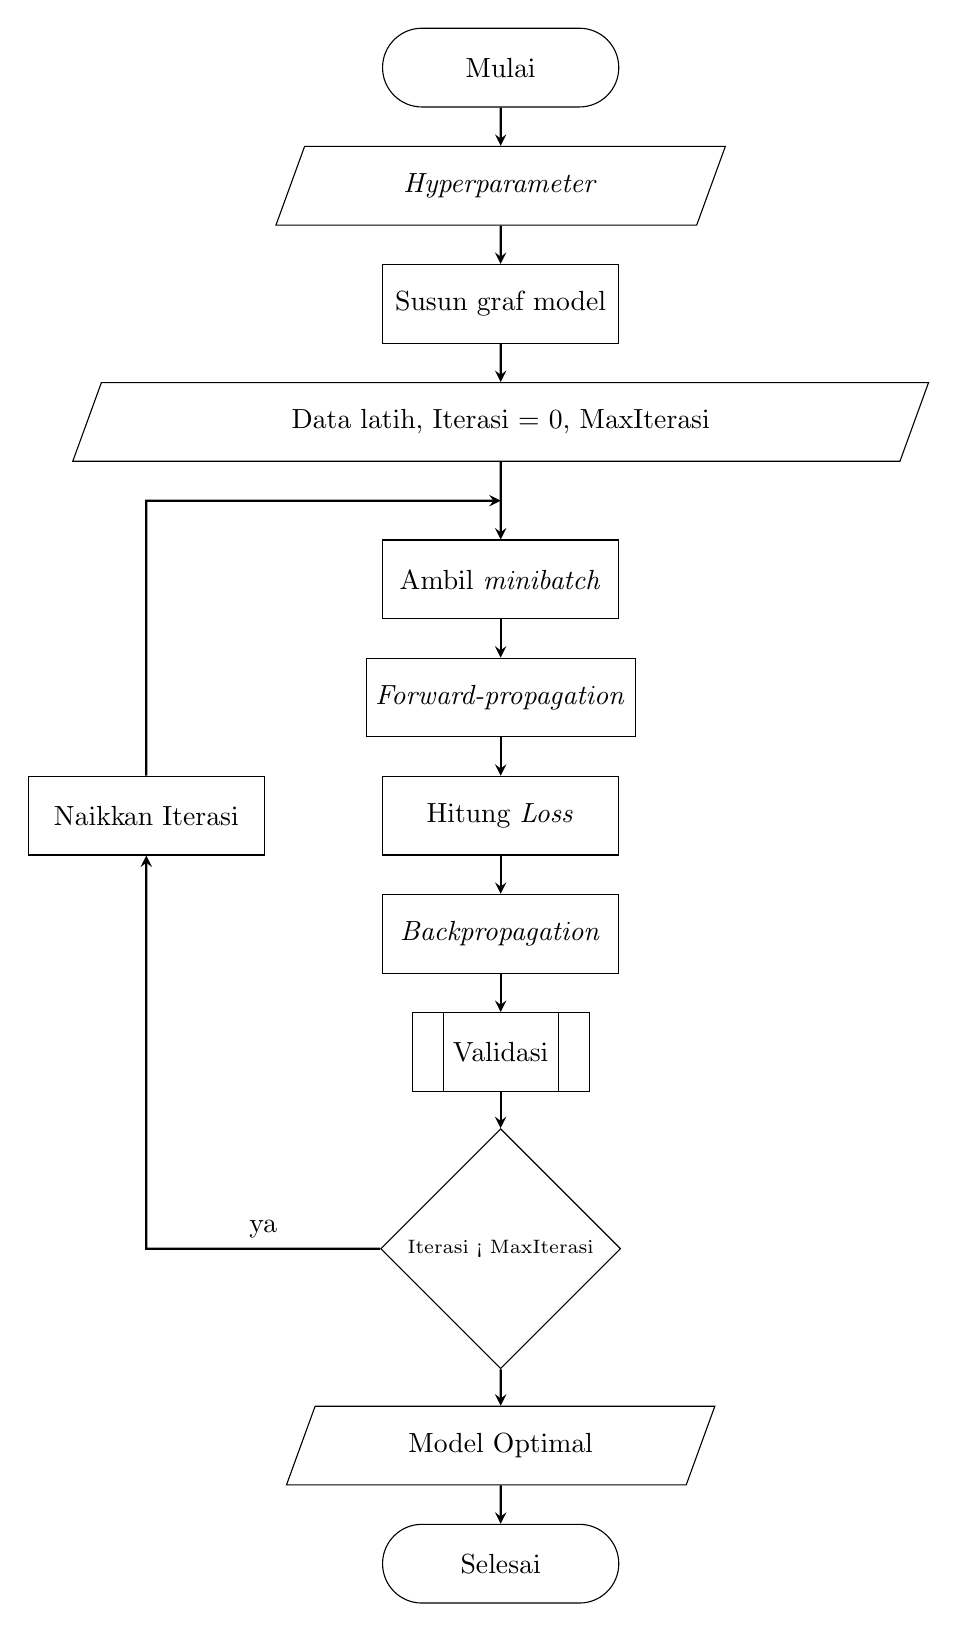
\begin{tikzpicture}[node distance=1.5cm]
            \node (mulai) [startstop] {Mulai};
            \node (hyperparameter) [io, below of=mulai] {\textit{Hyperparameter}};
            \node (graf) [process, below of=hyperparameter] {Susun graf model};
            \node (input) [io, below of=graf] {Data latih, Iterasi = 0, MaxIterasi};
            \node (minibatch) [process, below of=input, yshift=-0.5cm] {Ambil \textit{minibatch}};
            \node (forward-propagation) [process, below of=minibatch] {\textit{Forward-propagation}};
            \node (loss) [process, below of=forward-propagation] {Hitung \textit{Loss}};
            \node (backpropagation) [process, below of=loss] {\textit{Backpropagation}};
            \node (validasi) [external-process, below of=backpropagation] {\nodepart{two}\shortstack{Validasi}};
            \node (iterasi) [decision, below of=validasi, yshift=-1cm] {\scriptsize{Iterasi < MaxIterasi}};
            \node (increment) [process, left of=loss, xshift=-3cm] {Naikkan Iterasi};
            \node (output) [io, below of=iterasi, yshift=-1cm] {Model Optimal};
            \node (selesai) [startstop, below of=output] {Selesai};

            \draw [arrow] (mulai) -- (hyperparameter);
            \draw [arrow] (hyperparameter) -- (graf);
            \draw [arrow] (graf) -- (input);
            \draw [arrow] (input) -- (minibatch);
            \draw [arrow] (minibatch) -- (forward-propagation);
            \draw [arrow] (forward-propagation) -- (loss);
            \draw [arrow] (loss) -- (backpropagation);
            \draw [arrow] (iterasi) -- node[anchor=south] {ya} (-4.5,-15) -- (increment);
            \draw [arrow] (increment) -- (-4.5, -5.5) -- (0, -5.5);
            \draw [arrow] (backpropagation) -- (validasi);
            \draw [arrow] (validasi) -- (iterasi);
            \draw [arrow] (iterasi) -- (output);
            \draw [arrow] (output) -- (selesai);
        \end{tikzpicture}
    }
    \caption{Diagram alir proses pelatihan}
    \label{gambar:diagram-alir-pelatihan}
\end{figure}

Pada setiap iterasi pelatihan, \textit{minibatch} data diambil dari data latih dan dimasukkan sebagai input model. Lalu model melakukan \textit{forward propagation} untuk menghasilkan klasifikasi aktivitas dari setiap data pada \textit{minibatch}. \textit{Loss} dari hasil klasifikasi dihitung dengan \textit{cost function}. Berdasarkan \textit{loss} tersebut model dioptimasi dengan \textit{backpropagation}.

\textit{Cost function} yang digunakan adalah \textit{cross entropy}. Jika $x$ input, $a$ output jaringan dan $y$ output yang diinginkan, maka fungsi \textit{cross entropy} didefinisikan sebagai Persamaan~\ref{eq:cross-entropy} \Parencite{nielsen-2015}.

\begin{equation}
    C = -\frac{1}{n} \sum_{x}(y \ln{a} + (1 - y) \ln(1 - a))
    \label{eq:cross-entropy}
\end{equation}

Iterasi pelatihan juga malakukan proses validasi. Proses ini dilakukan untuk mengukur kemampuan model dalam mengklasifikasikan aktivitas pada data yang belum pernah ditemui sebelumnya. Diagram alir proses validasi dapat dilihat pada Gambar~\ref{gambar:diagram-alir-validasi}.

\begin{figure}[h]
    \centering
    \scalebox{0.8}{
        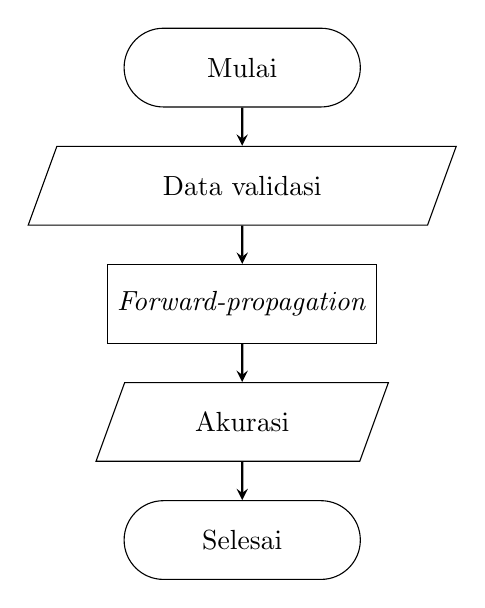
\begin{tikzpicture}[node distance=1.5cm]
            \node (mulai) [startstop] {Mulai};
            \node (data) [io, below of=mulai] {Data validasi};
            \node (forward-propagation) [process, below of=data] {\textit{Forward-propagation}};
            \node (akurasi) [io, below of=forward-propagation] {Akurasi};
            \node (selesai) [startstop, below of=akurasi] {Selesai};

            \draw [arrow] (mulai) -- (data);
            \draw [arrow] (data) -- (forward-propagation);
            \draw [arrow] (forward-propagation) -- (akurasi);
            \draw [arrow] (akurasi) -- (selesai);
        \end{tikzpicture}
    }
    \caption{Diagram alir proses validasi}
    \label{gambar:diagram-alir-validasi}
\end{figure}

Proses validasi menggunakan data validasi sebagai masukan model. \textit{Forward propagation} dilakukan pada data validasi untuk menghasilkan klasifikasi aktivitas. Kemudian hasil klasifikasi tersebut dibandingkan dengan label aktivitas pada dataset untuk mengukur akurasi. Pada akhir iterasi, parameter model optimal dipilih berdasarkan parameter yang menghasilkan akurasi terbaik pada proses validasi.

\section{Klasifikasi Pada Ponsel Cerdas}
Proses klasifikasi pada ponsel cerdas ditunjukkan pada Gambar~\ref{gambar:diagram-alir-klasifikasi-ponsel-cerdas}. Sensor akselerometer dan giroskop dibaca dengan \textit{sampling rate} 50 Hz. Masing-masing sensor menghasilkan data dengan tiga sumbu, sehingga satu kali pembacaan menghasilkan enam data. Hasil bacaannya dikumpulkan menjadi jendela berisi 100 sample dengan tumpang tindih 50\%. Dengan begitu, satu jendela data terdiri dari pembacaan sensor selama dua detik dan jendela baru dibuat setiap satu detik. Setelah jendela terpenuhi, jendela tersebut dijadikan sebagai masukan model klasifikasi yang telah dibuat. Proses ini menghasilkan kelas aktivitas manusia yang sesuai dengan bacaan sensor.

\begin{figure}[h]
    \centering
    \scalebox{0.8}{
        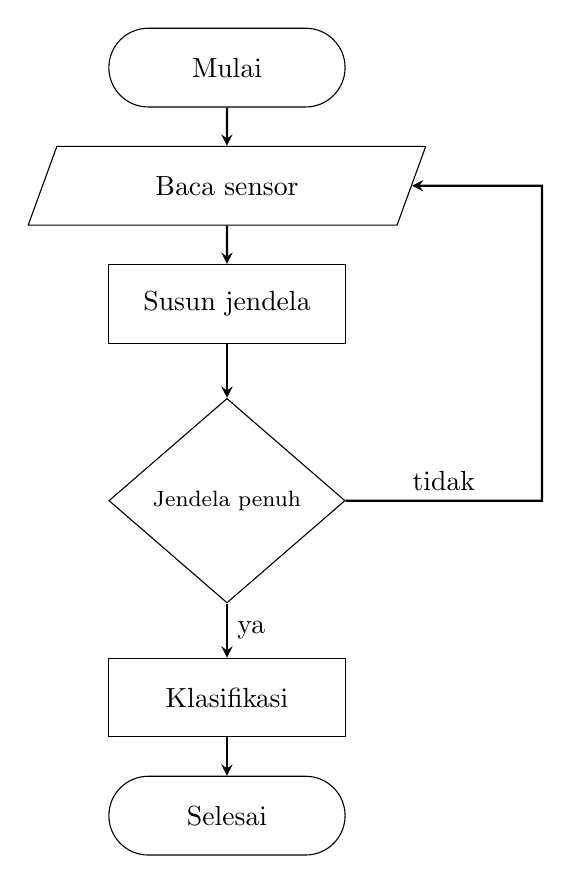
\begin{tikzpicture}[node distance=1.5cm]
            \node (mulai) [startstop] {Mulai};
            \node (baca-sensor) [io, below of=mulai] {Baca sensor};
            \node (susun-jendela) [process, below of=baca-sensor] {Susun jendela};
            \node (jendela-siap) [decision, below of=susun-jendela, yshift=-1cm] {\footnotesize{Jendela penuh}};
            \node (klasifikasi) [process, below of=jendela-siap, yshift=-1cm] {Klasifikasi};
            \node (selesai) [startstop, below of=klasifikasi] {Selesai};

            \draw [arrow] (mulai) -- (baca-sensor);
            \draw [arrow] (baca-sensor) -- (susun-jendela);
            \draw [arrow] (susun-jendela) -- (jendela-siap);
            \draw [arrow] (jendela-siap) -- node[anchor=south] {tidak} (4,-5.5) -- (4,-1.5) -- (baca-sensor);
            \draw [arrow] (jendela-siap) -- node[anchor=west] {ya} (klasifikasi);
            \draw [arrow] (klasifikasi) -- (selesai);
        \end{tikzpicture}
    }
    \caption{Diagram alir klasifikasi pada ponsel cerdas}
    \label{gambar:diagram-alir-klasifikasi-ponsel-cerdas}
\end{figure}

%------------------------------------------------------------------------------
% Pengujian
%
% Tabel: indikator keberhasilan
% Menjawab judul rumusan masalah
%------------------------------------------------------------------------------
\section{Rencana Pengujian}
Pengujian dilakukan untuk mengetahui kemampuan klasifikasi dari model yang telah dibuat. Terdapat dua pengujian yang dilakukan, yaitu pengujian \textit{hyperparameter} dan pengujian kecepatan klasifikasi pada ponsel cerdas. Kedua pengujian ini dilakukan dengan indikator pencapaian yang ditunjukkan pada Tabel~\ref{table:rencana-pengujian}.

{Pengujian} \textit{hyperparameter} dilakukan dengan diagram alir pada Gambar~\ref{gambar:diagram-alir-pengujian-hyperparameter}. Pada pengujian ini, model klasifikasi dengan berbagai variasi \textit{hyperparameter} diuji untuk mencari model paling optimal. Masing-masing variasi \textit{hyperparameter} memiliki nilai acak yang diambil dari distribusi seragam. Kemampuan model klasifikasi diukur berdasarkan akurasi klasifikasi pada data uji. Model menerima masukan data uji, lalu \textit{forward-propagation} dilakukan pada data uji untuk menghasilkan klasifikasi aktivitas. Kemudian akurasi diukur dengan membandingkan hasil klasifikasi dengan label aktivitas pada dataset.

\begin{figure}[h]
    \centering
    \scalebox{0.8}{
        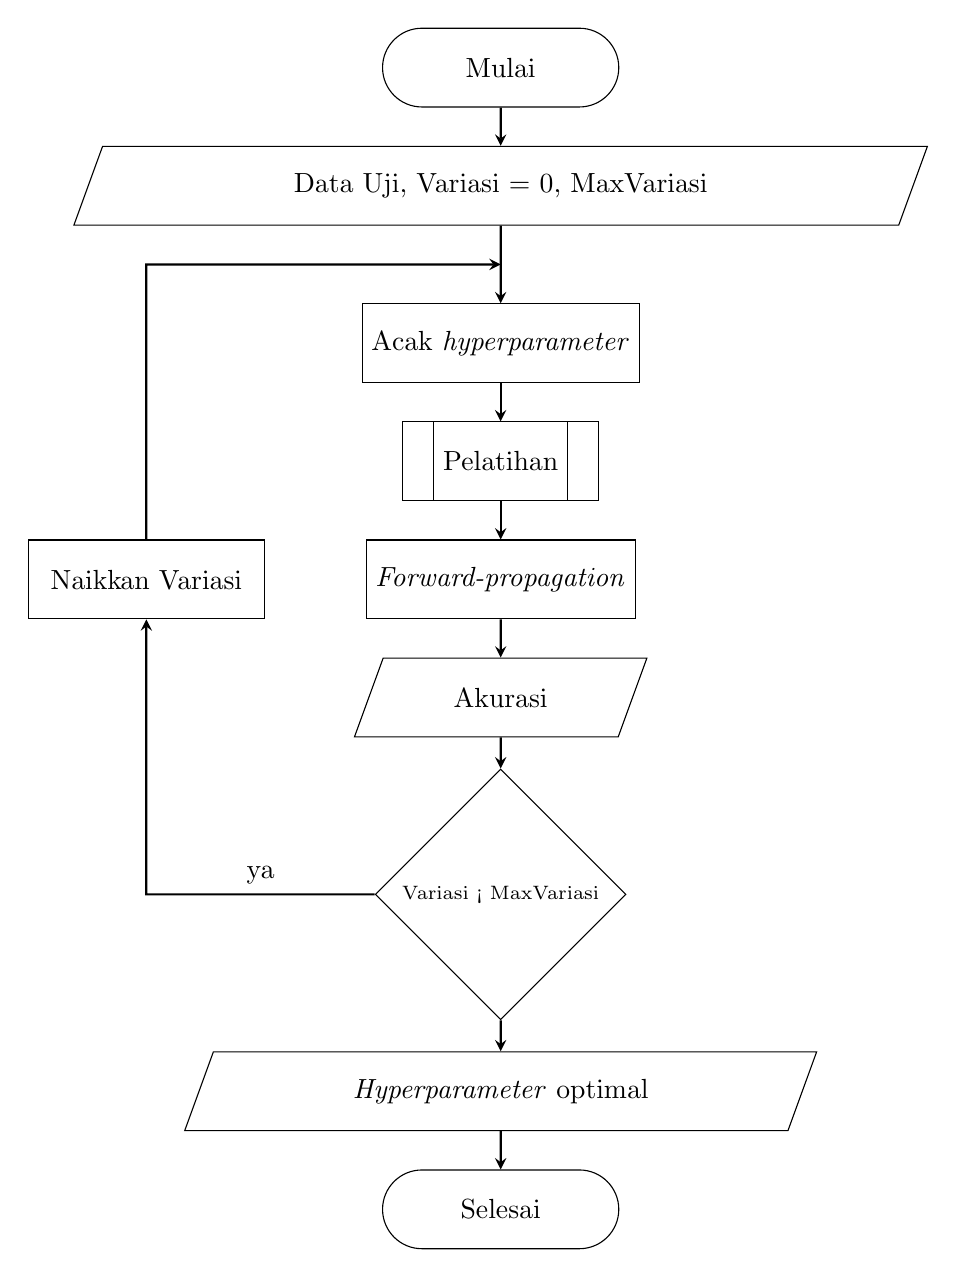
\begin{tikzpicture}[node distance=1.5cm]
            \node (mulai) [startstop] {Mulai};
            \node (input) [io, below of=mulai] {Data Uji, Variasi = 0, MaxVariasi};
            \node (acak-hyperparameter) [process, below of=input, yshift=-0.5cm] {Acak \textit{hyperparameter}};
            \node (latih) [external-process, below of=acak-hyperparameter] {\nodepart{two}\shortstack{Pelatihan}};
            \node (forward-propagation) [process, below of=latih] {\textit{Forward-propagation}};
            \node (akurasi) [io, below of=forward-propagation] {Akurasi};
            \node (iterasi) [decision, below of=akurasi, yshift=-1cm] {\scriptsize{Variasi < MaxVariasi}};
            \node (increment) [process, left of=forward-propagation, xshift=-3cm] {Naikkan Variasi};
            \node (output) [io, below of=iterasi, yshift=-1cm] {\textit{Hyperparameter} optimal};
            \node (selesai) [startstop, below of=output] {Selesai};

            \draw [arrow] (mulai) -- (input);
            \draw [arrow] (input) -- (acak-hyperparameter);
            \draw [arrow] (acak-hyperparameter) -- (latih);
            \draw [arrow] (latih) -- (forward-propagation);
            \draw [arrow] (forward-propagation) -- (akurasi);
            \draw [arrow] (akurasi) -- (iterasi);
            \draw [arrow] (iterasi) -- node[anchor=south] {ya} (-4.5,-10.5) -- (increment);
            \draw [arrow] (increment) -- (-4.5, -2.5) -- (0, -2.5);
            \draw [arrow] (iterasi) -- (output);
            \draw [arrow] (output) -- (selesai);
        \end{tikzpicture}
    }
    \caption{Diagram alir pengujian \textit{hyperparameter}}
    \label{gambar:diagram-alir-pengujian-hyperparameter}
\end{figure}

Pengujian kecepatan klasifikasi pada ponsel cerdas dilakukan dengan mengukur waktu yang dibutuhkan oleh setiap siklus klasifikasi, dimulai dari selesainya pengambilan data sensor sampai diperoleh kelas aktivitas dari data tersebut. Pengukuran ini dilakukan dengan beberapa jenis ponsel cerdas dengan kemampuan pemrosesan yang berbeda.

\begin{table}[h!]
    \centering
    \caption{Rencana Pengujian}
    \begin{tabular}{ |p{0.5cm}|p{5cm}|p{7.5cm}| }
        \hline
        \textbf{No} & \textbf{Parameter} & \textbf{Pencapaian} \\

        \hline
        1 & Pengujian \textit{hyperparameter} & Didapatkan \textit{hyperparameter} yang menghasilkan klasifikasi terbaik pada data uji \\
        
        \hline
        2 & Pengujian kecepatan klasifikasi pada ponsel cerdas & Klasifikasi dapat dilakukan secara \textit{realtime} pada ponsel cerdas \\

        \hline
    \end{tabular}
    \label{table:rencana-pengujian}
\end{table}

\chapter{IMPLEMENTASI}

\section{Implementasi Model Klasifikasi}
Model klasifikasi diimplementasikan dalam bahasa Python menggunakan pustaka TensorFlow. Model didefinisikan sebagai kelas \mintinline{python}{ConvLSTM} yang memperluas kelas \mintinline{python}{BaseModel}. Gambar~\ref{listing:har-ConvLSTM-constructor} menunjukkan \textit{constructor} dari kelas \mintinline{python}{ConvLSTM} dan Gambar~\ref{listing:har-BaseModel-constructor} menunjukkan \textit{constructor} kelas \mintinline{python}{BaseModel}.

\begin{figure}[h]
\begin{minted}[linenos=true,firstnumber=10]{python}
class ConvLSTM(BaseModel):
    def __init__(self, hyperparameter, logdir):
        super(ConvLSTM, self).__init__()

        self.hyperparameter = hyperparameter

        self.build_graph()

        self.session = tf.InteractiveSession(graph=self.target.graph)
        self.saver = Saver(self.session, logdir)

        self.session.run(tf.global_variables_initializer())
        self.session.run(tf.local_variables_initializer())
\end{minted}
\caption{\textit{Constructor} kelas ConvLSTM}
\label{listing:har-ConvLSTM-constructor}
\end{figure}

\begin{figure}[h]
\begin{minted}[linenos=true,firstnumber=10]{python}
class BaseModel(ABC):
    def __init__(self):
        self.session = None

        # Training placeholders
        self.input = tf.placeholder(tf.float32, [None, 600], name='input')
        self.target = tf.placeholder(tf.float32, [None, 6], name='target')

        self.output, self.train_op, self.accuracy_op = None, None, None
        self.saver = None
\end{minted}
\caption{\textit{Constructor} kelas BaseModel}
\label{listing:har-BaseModel-constructor}
\end{figure}

Pada \textit{constructor} tersebut didefinisikan beberapa atribut dari kelas \mintinline{python}{ConvLSTM}. Atribut \mintinline{python}{self.input} adalah atribut untuk menyimpan data sensor yang akan diklasifikasikan dan \mintinline{python}{self.target} adalah target aktivitas dari data tersebut. Atribut \mintinline{python}{self.input} menyimpan data sensor akselerometer dan giroskop sebagai matriks berukuran $1 \times 600$ dengan susunan

\begin{equation}
    \mintinline{python}{self.input} = [a_x^1, a_y^1, a_z^1, g_x^1, g_y^1, g_z^1,\dots, a_x^{100}, a_y^{100}, a_z^{100}, g_x^{100}, g_y^{100}, g_z^{100}]
    \label{eq:har-graph-input}
\end{equation}

\textit{Constructor} kelas \mintinline{python}{ConvLSTM} menerima dua argumen, \mintinline{python}{hyperparameter} dan \mintinline{python}{logdir}. Argumen \mintinline{python}{hyperparameter} adalah konfigurasi \textit{hyperparameter} yang digunakan untuk menyusun graf komputasi model. Pada argumen tersebut diatur beberapa hal berikut:

\begin{itemize}
    \item Pengaturan lapisan konvolusi (\mintinline{python}{hyperparameter.conv_layers}), meliputi jumlah lapisan, jumlah output dan ukuran kernel per lapisannya
    \item Pengaturan lapisan LSTM (\mintinline{python}{hyperparameter.lstm_layers}), meliputi jumlah lapisan dan jumlah unit LSTM per lapisannya
    \item Peluang \textit{dropout} (\mintinline{python}{hyperparameter.keep_prob})
    \item Laju pembelajaran (\mintinline{python}{hyperparameter.learning_rate})
\end{itemize}

Graf komputasi dibuat pada metode \mintinline{python}{self.build_graph()} dengan konfigurasi sesuai \textit{hyperparameter} yang telah diberikan. Metode tersebut diimplementasikan pada Gambar~\ref{listing:har-build-graph}.

\begin{figure}[h]
\begin{minted}[linenos=true,firstnumber=34]{python}
def build_graph(self):
    features = self.magnitude()
    conv_input = tf.reshape(features, [-1, 100, 8])
    conv = slim.stack(conv_input, slim.convolution, self.hyperparameter.conv_layers,
                      scope='conv')
    lstm = self._lstm_stack(conv)
    lstm_dropout = slim.dropout(lstm, self.hyperparameter.keep_prob,
                                is_training=self.is_training, scope='lstm_dropout')
    self.output = slim.fully_connected(lstm_dropout, 6, activation_fn=tf.nn.softmax,
                                    scope='output')
    self.train_op = self.create_train_op(self.hyperparameter.learning_rate)
    self.accuracy_op = self.create_accuracy_op()
\end{minted}
\caption{Implementasi penyusunan graf komputasi}
\label{listing:har-build-graph}
\end{figure}

Pada baris $35$, besar vektor input dihitung dengan metode \mintinline{python}{self.magnitude()}. Selanjutnya lapisan konvolusi didefinisikan pada baris $37$. Fungsi \mintinline{python}{slim.stack()} menerima input tensor \mintinline{python}{conv_input} dan membuat sejumlah lapisan konvolusi dengan konfigurasi sesuai dengan \mintinline{python}{self.hyperparameter.conv_layers}. Output dari lapisan konvolusi disimpan pada tensor \mintinline{python}{conv}.

Selanjutnya lapisan LSTM dibuat dengan memasukkan tensor \mintinline{python}{conv} ke metode \mintinline{python}{self._lstm_stack()} pada baris ke $39$. Metode tersebut diimplementasikan pada Gambar~\ref{listing:har-lstm-stack}. Baris $63$ sampai $64$ menyusun lapisan LSTM  sesuai dengan konfigurasi pada \mintinline{python}{self.hyperparameter.lstm_layers}. Output seluruh lapisan LSTM diambil dari langkah waktu terakhir pada lapisan LSTM terakhir.

\begin{figure}[h]
\begin{minted}[linenos=true,firstnumber=60]{python}
def _lstm_stack(self, tensor_in):
    with tf.name_scope('LSTM'):
        lstm_input = tf.transpose(tensor_in, [1, 0, 2])
        lstm = [tf.contrib.rnn.BasicLSTMCell(num_units) for num_units in
                self.hyperparameter.lstm_layers]
        lstm_cells = tf.contrib.rnn.MultiRNNCell(lstm)
        lstm_outputs, _ = tf.nn.dynamic_rnn(lstm_cells, lstm_input,
                                            dtype=tf.float32, time_major=True)

        return lstm_outputs[-1]
\end{minted}
\caption{Implementasi pembuatan lapisan LSTM}
\label{listing:har-lstm-stack}
\end{figure}

Output dari LSTM diregulasi dengan \textit{dropout} pada baris ke $40$. Lalu hasil \textit{dropout} masuk ke lapisan \textit{softmax} pada baris $42$. Lapisan \textit{softmax} ini menghasilkan distribusi probabilitas dari enam aktivitas yang diklasifikasikan. Output dari lapisan \textit{softmax} disimpan dalam \mintinline{python}{self.output}.

Graf pelatihan dibuat dengan memanggil metode  \mintinline{python}{self.create_train_op()} pada baris ke $44$. Metode tersebut diimplementasikan pada Gambar~\ref{listing:har-create-train-op}. Pada metode itu dihitung \textit{loss} dengan \textit{cross entropy}, lalu algoritme RMSProp digunakan untuk meminimalisir \textit{loss} tersebut. RMSProp digunakan dengan laju pembelajaran awal sesuai dengan \mintinline{python}{learning_rate} yang diatur pada \mintinline{python}{hyperparameter}. Selanjutnya graf pengukuran akurasi disusun dengan metode \mintinline{python}{self.create_accuracy_op()} yang diimplementasikan pada Gambar~\ref{listing:har-create-accuracy-op}.

\begin{figure}[h]
\begin{minted}[linenos=true,firstnumber=45]{python}
def create_train_op(self, learning_rate):
    loss = tf.losses.softmax_cross_entropy(self.target, self.output, scope='loss')

    with tf.name_scope('optimizer'):
        optimizer = tf.train.RMSPropOptimizer(learning_rate)
        return optimizer.minimize(loss)
\end{minted}
\caption{Implementasi pembuatan graf pelatihan}
\label{listing:har-create-train-op}
\end{figure}

\begin{figure}[h]
\begin{minted}[linenos=true,firstnumber=52]{python}
def create_accuracy_op(self):
with tf.name_scope('accuracy'):
    with tf.name_scope('correct_prediction'):
        correct_prediction = tf.equal(tf.argmax(self.output, 1),
                                      tf.argmax(self.target, 1))

    with tf.name_scope('accuracy'):
        accuracy = tf.reduce_mean(tf.cast(correct_prediction, tf.float32))
        tf.summary.scalar('accuracy', accuracy)

return accuracy
\end{minted}
\caption{Implementasi pengukuran akurasi}
\label{listing:har-create-accuracy-op}
\end{figure}

Proses pelatihan dilakukan dengan iterasi pada Gambar~\ref{listing:har-iterasi-pelatihan}. Baris 53 mengambil \textit{mini batch} untuk pelatihan dari dataset. Selanjutnya kondisi pada baris 55 menentukan agar instruksi pada baris $56-68$ dijalankan satu kali setiap \textit{epoch}. Pada baris $70-74$, seluruh graf pelatihan dijalankan. Data merambat dari node input ke setiap layer selanjutnya sampai ke output, lalu error dirambatkan ke belakang untuk mencari gradiennya. Dari gradien tersebut nilai parameter-parameter jaringan saraf dioptimasi untuk menghasilkan akurasi klasifikasi terbaik.

\begin{figure}[h]
\begin{minted}[linenos=true,firstnumber=52]{python}
for step in range(number_of_step):
    batch_features, batch_target = next(data_iterator)

    if step % one_epoch_step == 0 or step == number_of_step - 1:
        accuracy = self._evaluate(validation, merged_summary, step)
        best_accuracy, best_step = self._compare_accuracy(
            accuracy, best_accuracy, step, best_step)
        self.saver.save_checkpoint('last', step)

        early_stop = self._early_stop(
            self._step_to_epoch(step, data_length, batch_size),
            self._step_to_epoch(best_step, data_length, batch_size),
            10
        )

        if early_stop:
            break

    summary, _ = self.session.run([merged_summary, self.train_op], {
        self.input: batch_features,
        self.target: batch_target.eval(),
        self.is_training: True
    })
\end{minted}
\caption{Iterasi pelatihan}
\label{listing:har-iterasi-pelatihan}
\end{figure}

\section{Implementasi Pengujian \textit{Hyperparameter}}

Pengujian ini dilakukan dengan melatih model \mintinline{python}{ConvLSTM} dengan konfigurasi \textit{hyperparameter} yang berbeda, lalu menguji tingkat akurasi klasifikasi terhadap data uji. Implementasi pengujian ditunjukkan pada Gambar~\ref{listing:har-pengujian-hyperparameter}.

\begin{figure}[h]
\begin{minted}[linenos=true,firstnumber=108]{python}
def main(train_dataset=None, validation_dataset=None, test_dataset=None, epoch=30,
         batch_size=128, logdir=None, run=1, variation=1, checkpoint=None):
    hyperparameters = generate_hyperparameters(variation)
    for i, hyperparameter in enumerate(hyperparameters):
        run_logdir = os.path.join(logdir, 'run' + str(i + run))
        model = ConvLSTM(hyperparameter, run_logdir)
        print('Run %d/%d' % (i + 1, variation))
        print_hyperparameter_notes(hyperparameter)
        write_hyperparameter_notes(hyperparameter, run_logdir)

        if train_dataset and validation_dataset:
            train_data = load(train_dataset, NUM_TARGET, WINDOW_SIZE)
            validation_data = load(validation_dataset, NUM_TARGET, WINDOW_SIZE)

            if train_data.data.any() and validation_data.data.any():
                model.train(train_data, validation_data, epoch, batch_size,
                            checkpoint)

        if test_dataset:
            test_data = load(test_dataset, NUM_TARGET, WINDOW_SIZE)

            if test_data.data.any():
                prediction = model.test(test_data, batch_size, checkpoint)
                model.confusion_matrix(prediction, test_data.target)

        tf.reset_default_graph()
\end{minted}
\caption{Pengujian \textit{Hyperparameter}}
\label{listing:har-pengujian-hyperparameter}
\end{figure}

Pemilihan \textit{hyperparameter} dilakukan secara acak dengan memanggil fungsi \mintinline{python}{generate_hyperparameters()} pada baris 110. Argumen \mintinline{python}{variation} menentukan jumlah \textit{hyperparameter} yang akan dibuat. Pada baris 113 objek dari model \mintinline{python}{ConvLSTM} dibuat untuk setiap \textit{hyperparameter}. Data latih dan data validasi dibuka pada baris 119 dan 120, lalu model dilatih dengan memanggil \mintinline{python}{model.train()} pada baris 123. Setelah pelatihan model selesai, model diuji dengan data uji pada baris 127-133. Sebuah \textit{confusion matrix} dibuat dari hasil pengujian pada baris 131.

Implementasi fungsi \mintinline{python}{generate_hyperparameters()} dapat dilihat pada Gambar~\ref{listing:har-generate-hyperparameter}. Fungsi tersebut menerima argumen \mintinline{python}{variation} sebagai jumlah variasi \textit{hyperparameter} yang akan dibuat, lalu menghasilkan \textit{hyperparameter} acak dengan fungsi-fungsi berikut:

\begin{itemize}
    \item Fungsi \mintinline{python}{random_conv_layers()} untuk lapisan konvolusi
    \item Fungsi \mintinline{python}{random_lstm_layers()} untuk lapisan LSTM
    \item Fungsi \mintinline{python}{random_keep_prob()} untuk peluang dropout
    \item Fungsi \mintinline{python}{random_learning_rate()} untuk laju pembelajaran
\end{itemize}

\begin{figure}[h]
\begin{minted}[linenos=true,firstnumber=94]{python}
def generate_hyperparameters(variations, conv_layers=None, lstm_layers=None,
                             keep_prob=None, learning_rate=None):
    hyperparameters = []

    for _ in range(variations):
        hyperparameter = ConvLSTMHyperparameter(
            conv_layers if conv_layers else random_conv_layers(),
            lstm_layers if lstm_layers else random_lstm_layers(),
            keep_prob if keep_prob else random_keep_prob(0.2, 0.8),
            learning_rate if learning_rate else random_learning_rate(-4, -3)
        )
        hyperparameters.append(hyperparameter)

    return hyperparameters
\end{minted}
\caption{Pengujian \textit{Hyperparameter}}
\label{listing:har-generate-hyperparameter}
\end{figure}

Fungsi \mintinline{python}{random_conv_layers()} diimplementasikan pada Gambar~\ref{listing:har-random-conv-layers}. Pada fungsi tersebut dipilih variasi jumlah lapisan konvolusi antara 2 sampai 4 dan jumlah output masing-masing lapisan antara 32, 64 atau 128.

\begin{figure}[h]
\begin{minted}[linenos=false]{python}
def random_conv_layers():
    number_of_layers = np.random.randint(2, 5)
    num_outputs = np.random.choice([32, 64, 128])

    layers = []
    for _ in range(number_of_layers):
        layers.append((num_outputs, 5))

    return layers
\end{minted}
\caption{Pengacakan \textit{hyperparameter} lapisan konvolusi}
\label{listing:har-random-conv-layers}
\end{figure}

Fungsi \mintinline{python}{random_lstm_layers()} diimplementasikan pada Gambar~\ref{listing:har-random-lstm-layers}. Seperti pada fungsi \mintinline{python}{random_conv_layers()}, pada fungsi ini dipilih variasi jumlah lapisan LSTM antara 2 sampai 4 dan jumlah unit LSTM masing-masing lapisan antara 32, 64 atau 128.

\begin{figure}[h]
\begin{minted}[linenos=false]{python}
def random_lstm_layers():
    number_of_layers = np.random.randint(2, 5)
    num_units = np.random.choice([32, 64, 128])

    layers = []
    for _ in range(number_of_layers):
        layers.append(num_units)

    return layers
\end{minted}
\caption{Pengacakan \textit{hyperparameter} lapisan LSTM}
\label{listing:har-random-lstm-layers}
\end{figure}

Fungsi \mintinline{python}{random_keep_prob()} diimplementasikan pada Gambar~\ref{listing:har-random-keep-prob} dan fungsi \mintinline{python}{random_learning_rate()} diimplementasikan pada Gambar~\ref{listing:har-random-learning-rate}. Peluang dropout divariasikan antara 0,2 sampai 0,8, sedangkan laju pembelajaran divariasikan antara 0,0001 sampai 0,001.

\begin{figure}[h]
\begin{minted}[linenos=false]{python}
def random_keep_prob(kp_min, kp_max):
    return np.random.uniform(kp_min, kp_max)
\end{minted}
\caption{Pengacakan \textit{hyperparameter} peluang dropout}
\label{listing:har-random-keep-prob}
\end{figure}

\begin{figure}[h]
\begin{minted}[linenos=false]{python}
def random_learning_rate(lr_min, lr_max):
    return 10 ** np.random.uniform(lr_min, lr_max)
\end{minted}
\caption{Pengacakan \textit{hyperparameter} laju pembelajaran}
\label{listing:har-random-learning-rate}
\end{figure}

\section{Implementasi Pengujian Klasifikasi Online}

Pengujian klasifikasi online diimplementasikan pada ponsel cerdas Android. Proses klasifikasi dimulai dengan pengambilan dan pengondisian data sensor, kemudian data tersebut dijadikan sebagai input model \mintinline{python}{ConvLSTM}.

Data dari sensor diorganisir dalam dua kelas, yaitu kelas \mintinline{java}{SensorData} dan kelas \mintinline{java}{SensorDataSequence}. Kelas \mintinline{java}{SensorData} digunakan untuk menyimpan data sensor pada satu waktu, sedangkan kelas \mintinline{java}{SensorDataSequence} digunakan untuk menyimpan kumpulan \mintinline{java}{SensorData} pada langkah waktu yang berbeda.

Gambar~\ref{listing:aktvtas-sensordata} menunjukkan potongan implementasi kelas \mintinline{java}{SensorData}. Nilai sensor untuk masing-masing sumbu disimpan dalam sebuah \mintinline{java}{ArrayList}. Objek \mintinline{java}{SensorData} diinisialisasi dengan memberikan argumen \mintinline{java}{sensorType}, yang menyatakan jenis sensor, dan \mintinline{java}{numberOfAxis}, yang menyatakan jumlah sumbu pada jenis sensor tersebut. Selanjutnya nilai sensor dapat disimpan dengan memanggil metode \mintinline{java}{setValues()}.

\begin{figure}[h]
\begin{minted}[linenos=false]{java}
public class SensorData {
    private List<Float> values;
    private int sensorType;

    protected SensorData(int SensorType, int numberOfAxis) {
        this.sensorType = SensorType;

        Float[] initialData = new Float[numberOfAxis];
        values = Arrays.asList(initialData);
    }

    public void setValues(float[] values) {
        for (int i = 0; i < this.values.size(); i++) {
            this.values.set(i, values[i]);
        }
    }
    ...
}
\end{minted}
\caption{Potongan Kelas SensorData}
\label{listing:aktvtas-sensordata}
\end{figure}

Kelas \mintinline{java}{SensorDataSequence} diimplementasikan pada Gambar~\ref{listing:aktvtas-sensordatasequence}. Rangkaian data sensor disimpan dalam \mintinline{java}{ArrayList} berisi \mintinline{java}{SensorData} yang bernama \mintinline{java}{sequence}. Sebuah \mintinline{java}{buffer} digunakan untuk penyimpanan data sensor sementara selama proses pengisian masih berlangsung. Kelas tersebut juga menyimpan referensi terhadap jumlah sensor yang didaftarkan pada atribut \mintinline{java}{registeredSensor}, dan urutan \mintinline{java}{SensorData} pada \mintinline{java}{buffer} disimpan dalam \mintinline{java}{sensorOrder}.

\begin{figure}[h!]
\begin{minted}[linenos=false]{java}
public class SensorDataSequence {
    List<SensorData> buffer = new ArrayList<>();
    protected List<List<SensorData>> sequence = new ArrayList<>();
    HashMap<Integer, Integer> sensorOrder = new HashMap<>();
    private int registeredSensor = 0;
    
    public SensorDataSequence registerSensor(SensorData sensorData) {
        sensorOrder.put(sensorData.sensorType(), registeredSensor++);
        buffer.add(sensorData);

        return this;
    }

    public SensorDataSequence setData(SensorData sensorData) {
        int index = sensorOrder.get(sensorData.sensorType());

        SensorData newSensorData = new SensorData(sensorData.sensorType(),
                                                  sensorData.numberOfAxis());
        newSensorData.setValues(sensorData.getValues());
        buffer.set(index, newSensorData);

        return this;
    }

    public void commit() {
        if (! dataCorrupted()) {
            sequence.add(buffer);
        }
        resetBuffer();
    }
}
\end{minted}
\caption{Potongan Kelas SensorDataSequence}
\label{listing:aktvtas-sensordatasequence}
\end{figure}

Sebelum digunakan, \mintinline{java}{buffer} perlu diinisialisasi dengan mendaftarkan seluruh jenis sensor yang datanya akan disimpan. Pendaftaran ini dilakukan dengan memanggil metode \mintinline{java}{registerSensor()} dan memberikan argumen \mintinline{java}{SensorData}. Setelah pendaftaran seluruh sensor selesai, data sensor pada \mintinline{java}{buffer} dapat diisi dengan memberikan \mintinline{java}{SensorData} pada metode \mintinline{java}{setData()}. Ketika data seluruh jenis sensor pada satu langkah waktu telah selesai diisikan pada \mintinline{java}{buffer}, data dapat disusun pada \mintinline{java}{sequence} dengan memanggil metode \mintinline{java}{commit()}. Selain menyimpan  \mintinline{java}{buffer} pada urutan langkah waktu dalam \mintinline{java}{sequence}, metode tersebut juga mereset \mintinline{java}{buffer} agar siap digunakan pada langkah waktu selanjutnya.

Pembacaan sensor dilakukan oleh kelas \mintinline{java}{SensorReader} yang diimplementasikan pada Gambar~\ref{listing:aktvtas-sensorreader}. Pada \textit{constructor} kelas \mintinline{java}{SensorReader}, seluruh sensor yang diberikan pada argumen \mintinline{java}{sensorToRead} diinisialisasi dengan memanggil metode \mintinline{java}{registerSensorIfAvailable()}. Metode tersebut mendaftarkan sensor pada \textit{listener} dalam sistem operasi Android, sehingga sensor dapat dibaca. Kelas \mintinline{java}{SensorReader} juga memiliki atribut \mintinline{java}{sensorDataBuffer} sebagai penyimpanan sementara selama proses pembacaan pada satu langkah waktu dilakukan.

\begin{figure}[h]
\begin{minted}[linenos=false]{java}
public class SensorReader implements SensorEventListener {
    private final SensorManager sensorManager;
    private List<Sensor> availableSensors = new ArrayList<>();
    private List<SensorData> sensorDataBuffer;

    public SensorReader(Context context, List<Integer> sensorToRead) {
        sensorManager = (SensorManager) context.getSystemService(
            Context.SENSOR_SERVICE);

        for (Integer sensorType : sensorToRead) {
            registerSensorIfAvailable(sensorType);
        }
        resetBuffer();
    }

    private void registerSensorIfAvailable(int sensorType) {
        if (sensorManager.getDefaultSensor(sensorType) != null) {
            Sensor sensor = sensorManager.getDefaultSensor(sensorType);
            sensorManager.registerListener(this, sensor,
                                           SensorManager.SENSOR_DELAY_GAME);
            availableSensors.add(sensor);
        }
    }
    ...
}
\end{minted}
\caption{Potongan Kelas SensorReader}
\label{listing:aktvtas-sensorreader}
\end{figure}

Perubahan data sensor yang telah didaftarkan memicu dipanggilnya metode \mintinline{java}{onSensorChanged()} yang diimplementasikan pada Gambar~\ref{listing:aktvtas-pembacaan-sensorreader}. Pada metode tersebut dibuat objek \mintinline{java}{SensorData} sesuai dengan jenis data sensor yang baru diterima, lalu data baru tersebut disimpan pada \mintinline{java}{SensorData} dengan memanggil metode \mintinline{java}{sensorData.setValues()}. Selanjutnya objek \mintinline{java}{SensorData} tersebut disimpan dalam \mintinline{java}{sensorDataBuffer}.

\begin{figure}[h]
\begin{minted}[linenos=false]{java}
public class SensorReader implements SensorEventListener {
    ...
    @Override
    public final void onSensorChanged(SensorEvent event) {
        storeAvailableSensorDataToBuffer(event);

        if (readyToRead() && sensorReaderEvent != null) {
            sensorReaderEvent.onSensorDataReady();
        }
    }

    void storeAvailableSensorDataToBuffer(SensorEvent event) {
        if (availableSensors.contains(event.sensor)) {
            int bufferIndex = availableSensors.indexOf(event.sensor);
            SensorData sensorData = new SensorData(event.sensor.getType(),
                                                   event.values.length);
            sensorData.setValues(event.values);
            sensorDataBuffer.set(bufferIndex, sensorData);
        }
    }
    ...
}
\end{minted}
\caption{Pembacaan sensor pada SensorReader}
\label{listing:aktvtas-pembacaan-sensorreader}
\end{figure}

\begin{figure}[h!]
\begin{minted}[linenos=false]{java}
public class SensorReader implements SensorEventListener {
    ...
    public boolean readyToRead() {
        for (SensorData buffer : sensorDataBuffer) {
            if (buffer == null) {
                return false;
            }
        }
        return true;
    }

    public List<SensorData> read() {
        if (readyToRead()) {
            List<SensorData> sensorDataList = new ArrayList<>(sensorDataBuffer);
            resetBuffer();
            return sensorDataList;
        } else {
            return new ArrayList<>();
        }
    }
    ...
\end{minted}
\caption{Pengambilan data dari SensorReader}
\label{listing:aktvtas-pengambilan-sensorreader}
\end{figure}

Apabila \mintinline{java}{sensorDataBuffer} telah dipenuhi oleh data setiap sensor pada satu langkah waktu, data dapat diambil dengan memanggil metode \mintinline{java}{read()} yang diimplementasikan pada Gambar~\ref{listing:aktvtas-pengambilan-sensorreader}. Selain mengembalikan data dari seluruh sensor yang dibaca, metode tersebut juga mengosongkan \mintinline{java}{sensorDataBuffer} untuk penggunaan pada langkah waktu selanjutnya. Adapun penentuan siap atau tidaknya data diambil dari \mintinline{java}{sensorDataBuffer} dilakukan oleh metode \mintinline{java}{readyToRead()} yang memeriksa setiap anggota \mintinline{java}{sensorDataBuffer}. Jika sudah tidak terdapat anggota yang kosong, pengambilan data dapat dilakukan.

Kelas \mintinline{java}{SensorReader} juga menyediakan \textit{interface} \mintinline{java}{SensorReaderEvent} seperti yang ditunjukkan pada Gambar~\ref{listing:aktvtas-sensorreaderevent}. \textit{Interface} ini dapat diimplementasikan oleh kelas lain untuk menerima fungsi \textit{callback} \mintinline{java}{onSensorDataReady()} yang dipanggil ketika data sensor pada satu langkah waktu telah siap digunakan.

\begin{figure}[h]
\begin{minted}[linenos=false]{java}
public class SensorReader implements SensorEventListener {
    ...
    private SensorReaderEvent sensorReaderEvent;

    public interface SensorReaderEvent {
        void onSensorDataReady();
    }

    public void enableEventCallback(SensorReaderEvent event) {
        sensorReaderEvent = event;
    }
    ...
}
\end{minted}
\caption{\textit{Interface} SensorReaderEvent pada SensorReader}
\label{listing:aktvtas-sensorreaderevent}
\end{figure}

Rutin pengambilan data sensor dilakukan dengan \textit{service} \mintinline{java}{SensorService} yang diimplementasikan pada Gambar~\ref{listing:aktvtas-sensorservice}. Kelas ini mengimplementasikan \textit{interface} \mintinline{java}{SensorReader.SensorReaderEvent}, sehingga dapat menerima \textit{callback} \mintinline{java}{onSensorDataReady()} ketika data sensor telah selesai dibaca.

\begin{figure}[h]
\begin{minted}[linenos=false]{java}
public class SensorService extends Service
                           implements SensorReader.SensorReaderEvent {
    protected int entryCounter = 0;
    private List<SensorData> buffer;
    protected SensorReader sensorReader;
    protected SensorDataSequence sensorDataSequence;

    protected void createSensorDataReader(List<Integer> sensorToRead) {
        sensorReader = new SensorReader(this, sensorToRead);
        sensorReader.enableEventCallback(this);
    }

    protected void createSensorDataSequence(List<Integer> sensorToRead,
                                            List<Integer> numberOfAxis) {
        sensorDataSequence = SensorDataSequence.create(sensorToRead, numberOfAxis);
    }

    @Override
    public void onSensorDataReady() {
        buffer = sensorReader.read();
        if (buffer != null) {
            for (SensorData data : buffer) {
                sensorDataSequence.setData(data);
            }
            sensorDataSequence.commit();
            entryCounter++;
        }
    }
    ...
}
\end{minted}
\caption{Kelas SensorService}
\label{listing:aktvtas-sensorservice}
\end{figure}

Kelas \mintinline{java}{SensorService} memiliki atribut dari kelas \mintinline{java}{SensorReader} dan kelas \mintinline{java}{SensorDataSequence}. Keduanya diinisialisasi secara berurutan dengan memanggil metode \mintinline{java}{createSensorDataReader()} dan \mintinline{java}{createSensorDataSequence()}. Pada fungsi \textit{callback} \mintinline{java}{onSensorDataReady()}, sensor dibaca dengan memanggil \mintinline{java}{sensorReader.read()}, lalu hasilnya disusun dalam \mintinline{java}{SensorDataSequence} dengan memasukkan data sensor ke \mintinline{java}{sensorDataSequence.setData(data)}.

Rutin klasifikasi aktivitas dilakukan dengan \textit{service} \mintinline{java}{PredictionService} yang memperluas \mintinline{java}{SensorService}. Implementasi \mintinline{java}{PredictionService} dapat dilihat pada Gambar~\ref{listing:aktvtas-predictionservice}.

\begin{figure}[h!]
\begin{minted}[linenos=false]{java}
public class PredictionService extends SensorService {
    private HumanActivityClassifier classifier;
    private List<Recognition> lastRecognitions;
    private int totalPrediction = 0;
    private int correctPrediction = 0;
    private long totalPredictionTime = 0;
    private float accuracy = 0f;

    @Override
    public void onSensorDataReady() {
        super.onSensorDataReady();

        if (sensorDataSequence.size() == windowSize) {
            long startTime = System.currentTimeMillis();

            List<Recognition> recognitions = classifier.classify(
                sensorDataSequence);

            long predictionTime = System.currentTimeMillis() - startTime;
            totalPredictionTime += predictionTime;

            if (! recognitions.equals(lastRecognitions)) {
                reportPredictions(recognitions);
                lastRecognitions = recognitions;
            }
            totalPrediction += 1;

            if (recognitions.size() > 0) {
                if (recognitions.get(0).getId() == acquisition.getActivityId()
                    .ordinal()) {
                    correctPrediction += 1;
                }
                if (correctPrediction > 0) {
                    accuracy = ((float) correctPrediction / (float) totalPrediction) * 100;
                }
            }

            logWriter.write(recognitions.get(0).getId(), predictionTime);
            rearrangeSequence();
        }
    }
    ...
}
\end{minted}
\caption{Kelas PredictionService}
\label{listing:aktvtas-predictionservice}
\end{figure}

Implementasi fungsi \mintinline{java}{onSensorDataReady()} kelas \mintinline{java}{PredictionService} menjalankan instruksi \mintinline{java}{super.onSensorDataReady()}. Hal ini dilakukan untuk menjalankan implementasi \mintinline{java}{onSensorDataReady()} pada kelas \mintinline{java}{SensorService}, sehingga rangkaian data sensor diisi pada \mintinline{java}{sensorDataSequence}. Setelah panjang rangkaian \mintinline{java}{sensorDataSequence} sesuai dengan panjang jendela yang diinginkan, proses klasifikasi dimulai.

Klasifikasi dilakukan dengan memasukkan \mintinline{java}{sensorDataSequence} pada metode \mintinline{java}{classifier.classify()}. Metode tersebut mengembalikan \mintinline{java}{ArrayList} berisi persebaran peluang kelas aktivitas, diurutkan dari kelas aktivitas dengan peluang terbesar sampai terkecil. Perhitungan akurasi dilakukan dengan membandingkan prediksi aktivitas berpeluang terbesar dengan referensi aktivitas. Setelah proses klasifikasi selesai, data pada \mintinline{java}{sensorDataSequence} disusun ulang mengikuti aturan \textit{sliding window} dengan memanggil metode \mintinline{java}{rearrangeSequence()}. Metode tersebut mengambil sebagian data \mintinline{java}{sensorDataSequence} terakhir, lalu pengisian data dilanjutkan pada potongan baru tersebut. Aturan ini mengikuti parameter \textit{sliding window} yang diberikan. Selama \textit{service} \mintinline{java}{PredictionService} dijalankan, akurasi akan terus diperbarui dengan prediksi aktivitas terbaru. Selain itu hasil klasifikasi pada setiap langkah waktu disimpan dalam sebuah file dengan metode \mintinline{java}{logWriter.write()}.

Atribut \mintinline{java}{classifier} yang digunakan untuk mengklasifikasikan aktivitas merupakan objek dari kelas \mintinline{java}{HumanActivityClassifier}. Implementasi kelas tersebut dapat dilihat pada Gambar~\ref{listing:aktvtas-humanactivityclassifier}. Proses klasifikasi dilakukan dengan metode \mintinline{java}{classify()}. Data pada parameter \mintinline{java}{sequence} diratakan menjadi array seperti pada Persamaan~\ref{eq:har-graph-input} dengan memanggil metode \mintinline{java}{flatten()} dari \mintinline{java}{sensorDataSequence}. Kemudian data yang telah diratakan dimasukkan pada graf komputasi yang dimuat dari \mintinline{java}{MODEL_FILE}. Instuksi \mintinline{java}{inferenceInterface.run()} merambatkan data pada jaringan yang telah disusun. Komputasi pada graf tersebut menghasilkan distribusi peluang kelas aktivitas dari output lapisan \textit{softmax}. Lalu hasil klasifikasi diurutkan berdasarkan peluang terbesar dengan metode \mintinline{java}{findBestClassification()}.

\begin{figure}[h!]
\begin{minted}[linenos=false]{java}
public class HumanActivityClassifier {
    private static final String MODEL_FILE = "file:///android_asset/graph.pb";

    private static final String INPUT_NAME = "input:0";
    private static final String OUTPUT_NAME = "output/Softmax:0";

    private TensorFlowInferenceInterface inferenceInterface;

    public HumanActivityClassifier(AssetManager assetManager) {
        inferenceInterface = new TensorFlowInferenceInterface(assetManager,
                                                              MODEL_FILE);
    }

    public List<Recognition> classify(SensorDataSequence sequence) {
        float inputNode[] = sequence.flatten();

        inferenceInterface.feed(INPUT_NAME, inputNode, 600);
        inferenceInterface.run(new String[] {OUTPUT_NAME});
        inferenceInterface.fetch(OUTPUT_NAME, outputs);

        return findBestClassification(outputs);
    }
}
\end{minted}
\caption{Kelas HumanActivityClassifier}
\label{listing:aktvtas-humanactivityclassifier}
\end{figure}

\section{Implementasi Pengujian Kecepatan Klasifikasi pada Ponsel Cerdas}

Pengujian kecepatan klasifikasi pada ponsel cerdas dilakukan bersamaan dengan pengujian klasifikasi online. Pada kelas \mintinline{java}{PredictionService} dalam metode \mintinline{java}{onSensorDataReady()} (Gambar~\ref{listing:aktvtas-predictionservice}), diukur waktu yang dibutuhkan untuk menjalankan instruksi \mintinline{java}{classifier.classify()}. Waktu yang diperoleh kemudian disimpan dalam file dengan instruksi \mintinline{java}{logWriter.write()}. Pengukuran ini dilakukan selama \mintinline{java}{PredictionService} berjalan.

\chapter{HASIL DAN PEMBAHASAN}

\section{Pengujian Hyperparameter}

Pengujian \textit{hyperparameter} dilakukan untuk mencari model klasifikasi terbaik, yaitu model yang memenuhi beberapa kriteria berikut:

\begin{enumerate}
    \item Model dapat melakukan klasifikasi dengan baik, ditunjukkan dengan tingkat akurasi klasifikasi yang tinggi terhadap data uji.
    \item Model dapat menyamaratakan dengan baik, ditunjukkan dengan perbedaan yang tidak signifikan antara akurasi klasifikasi data latih dengan akurasi data validasi dan data uji.
    \item Kompleksitas model minimal, sehingga mengurangi beban komputasi dan klasifikasi dapat dilakukan secara \textit{realtime} pada ponsel cerdas.
\end{enumerate}

Variasi \textit{hyperparameter} ditunjukkan pada Tabel~\ref{table:variasi-hyperparameter}. Pengujian dilakukan sebanyak 31 kali dengan variasi \textit{hyperparameter} yang dipilih secara acak. Masing-masing variasi dilatih dalam maksimal 30 \textit{epoch}.

\begin{table}[h!]
    \centering
    \caption{Variasi hyperparameter}
    \begin{tabular}{ |l|c| }
        \hline
        Hyperparameter & Variasi \\

        \hline
        Jumlah lapisan konvolusi & $2 - 4$ \\

        \hline
        Jumlah output konvolusi & $32, 64, 128$ \\

        \hline
        Jumlah lapisan LSTM & $2 - 4$ \\

        \hline
        Jumlah unit LSTM & $32, 64, 128$ \\

        \hline
        Peluang \textit{dropout} & $0,2 - 0,8$ \\

        \hline
        Laju pembelajaran ($\alpha$) & $10^{-4} - 10^{-3}$ \\

        \hline
    \end{tabular}
    \label{table:variasi-hyperparameter}
\end{table}

Hasil pengujian dapat dilihat pada Tabel~\ref{table:hasil-pengujian-hyperparameter}. Perbedaan \textit{hyperparameter} yang digunakan menghasilkan tingkat akurasi klasifikasi yang berbeda. Berdasarkan hasil tersebut, diambil tiga \textit{hyperparameter} dengan akurasi terbaik untuk dibandingkan lebih lanjut, yaitu \textit{hyperparameter} pada variasi nomor 8, 17 dan 28.

\begin{table}[h!]
    \centering
    \caption{Hasil pengujian \textit{hyperparameter}}
    \pgfplotstabletypeset[
        col sep=comma,
        before row=\hline,every last row/.style={after row=\hline},
        display columns/0/.style={column type=|c|},
        display columns/1/.style={string type, column type=l|},
        display columns/2/.style={string type, column type=l|},
        display columns/3/.style={column type=c|},
        display columns/4/.style={column type=c|,column name=$\alpha$},
        display columns/5/.style={column type=c|,precision=5},
    ]{data/pelatihan/hyperparameter.csv}
    \label{table:hasil-pengujian-hyperparameter}
\end{table}

Variasi 8 menggunakan empat lapisan konvolusi dan empat lapisan LSTM\@. Keempat lapisan konvolusi menggunakan kernel dengan $64$ output. Lapisan konvolusi pertama menerima input tensor dengan dimensi $100 \times 8$ dan lapisan konvolusi terakhir menghasilkan output tensor dengan ukuran $100 \times 64$. Keempat lapisan LSTM memiliki $32$ unit LSTM\@. Lapisan LSTM pertama menerima input tensor dari output konvolusi dan lapisan LSTM terakhir menghasilkan output tensor dengan ukuran $1 \times 32$. Variasi ini dilatih dengan peluang \textit{dropout} $0.79$ dan laju pembelajaran $1.46 \times 10^{-4}$.

Proses pelatihan variasi 8 dapat dilihat pada Gambar~\ref{gambar:run8-training}. Grafik tersebut menunjukkan peningkatan akurasi klasifikasi dalam proses pelatihan terhadap data latih dan data validasi. Model akhir diambil dari kondisi jaringan saat menghasilkan akurasi terbaik terhadap data validasi, yaitu pada iterasi ke $5069$ dengan akurasi $0.912331$. Pada iterasi yang sama, akurasi terhadap data latih adalah $0.982142$ dan akurasi terhadap data uji adalah $0.91169$.

\begin{figure}[h!]
    \centering
    \includegraphics[width=14cm]{data/pelatihan/run8-accuracy.png}
    \caption{Proses pelatihan pada variasi 8}.
    \label{gambar:run8-training}
\end{figure}

\textit{Confusion matrix} variasi 8 dapat dilihat pada Gambar~\ref{gambar:run8-confusion-martix}. Pada gambar tersebut dapat dilihat bahwa klasifikasi dilakukan dengan baik pada aktivitas berdiri (96,9\%), duduk (94,9\%) dan lari (96,9\%). Aktivitas jalan memiliki akurasi 87,6\% dan \textit{false negative} yang cukup besar pada naik tangga (8,5\%) dan turun tangga (3,9\%). Aktivitas naik dan turun tangga memiliki klasifikasi terburuk dengan akurasi masing-masing 78,6\% dan 78,4\%, dengan \textit{false negative} tersebar pada seluruh aktivitas lainnya.

\begin{figure}[h!]
    \centering
    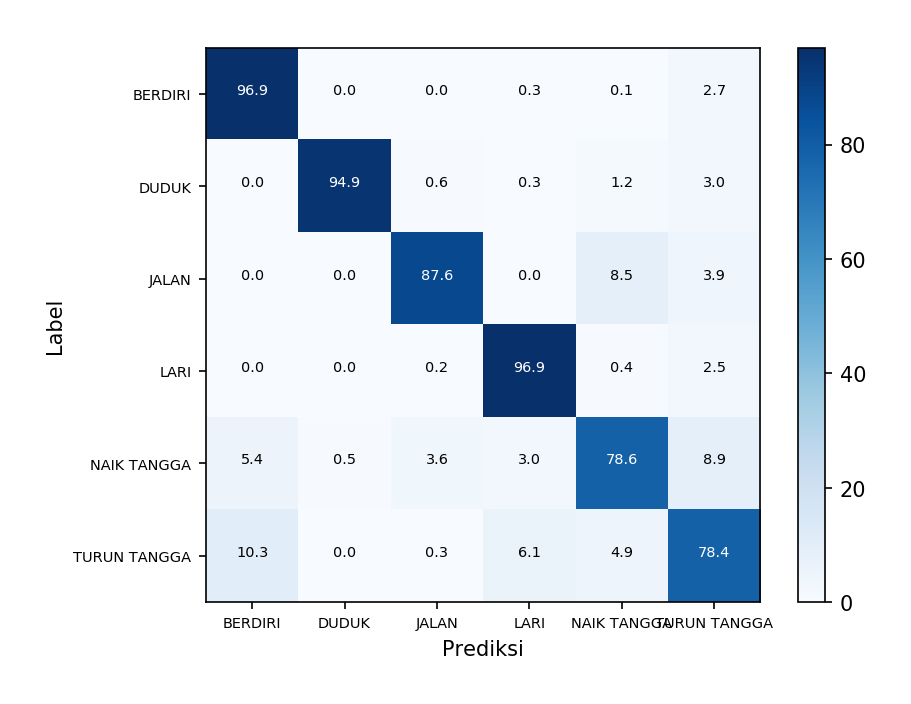
\includegraphics[width=13cm]{gambar/hasil-pembahasan/run8-confusion-matrix.png}
    \caption{\textit{Confusion matrix} pada variasi 8}.
    \label{gambar:run8-confusion-martix}
\end{figure}

Variasi 17 menggunakan tiga lapisan konvolusi dan tiga lapisan LSTM\@. Masing-masing lapisan konvolusi menggunakan kernel dengan $64$ output. Lapisan konvolusi pertama menerima input tensor dengan dimensi $100 \times 8$ dan lapisan konvolusi terakhir menghasilkan output tensor dengan ukuran $100 \times 64$. Masing-masing lapisan LSTM memiliki $64$ unit LSTM\@. Lapisan LSTM pertama menerima input tensor dari output konvolusi dan lapisan LSTM terakhir menghasilkan output tensor dengan ukuran $1 \times 64$. Variasi ini dilatih dengan peluang \textit{dropout} $0.59$ dan laju pembelajaran $2.81 \times 10^{-4}$.

Proses pelatihan variasi 17 dapat dilihat pada Gambar~\ref{gambar:run17-training}. Model akhir diambil dari kondisi jaringan saat menghasilkan akurasi terbaik terhadap data validasi, yaitu pada iterasi ke $4394$ dengan akurasi $0.929793$. Pada iterasi yang sama, akurasi terhadap data latih adalah $1.0$ dan akurasi terhadap data uji  $0.93652$.

\begin{figure}[h!]
    \centering
    \includegraphics[width=14cm]{data/pelatihan/run17-accuracy.png}
    \caption{Proses pelatihan pada variasi 17}.
    \label{gambar:run17-training}
\end{figure}

\textit{Confusion matrix} variasi 17 dapat dilihat pada Gambar~\ref{gambar:run17-confusion-martix}. Pada gambar tersebut dapat dilihat bahwa klasifikasi dilakukan dengan baik pada aktivitas berdiri (97,2\%), duduk (93,4\%) dan jalan (96,1\%). Aktivitas lari memiliki akurasi 85,5\% dan \textit{false negative} yang cukup besar pada jalan (8,6\%) dan turun tangga (5,7\%). Aktivitas naik dan turun tangga memiliki akurasi masing-masing 81,2\% dan 82,4\%, dengan \textit{false negative} tersebar pada seluruh aktivitas lainnya.

\begin{figure}[h!]
    \centering
    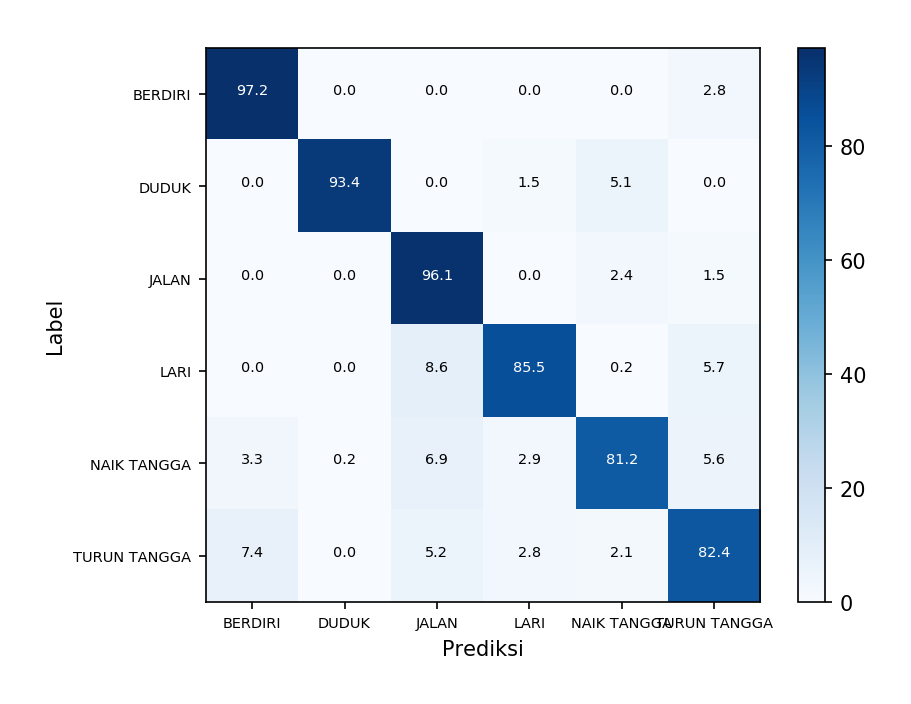
\includegraphics[width=13cm]{gambar/hasil-pembahasan/run17-confusion-matrix.png}
    \caption{\textit{Confusion matrix} pada variasi 17}.
    \label{gambar:run17-confusion-martix}
\end{figure}

Variasi 28 menggunakan empat lapisan konvolusi dan tiga lapisan LSTM\@. Masing-masing lapisan konvolusi menggunakan kernel dengan $64$ output. Lapisan konvolusi pertama menerima input tensor dengan dimensi $100 \times 8$ dan lapisan konvolusi terakhir menghasilkan output tensor dengan ukuran $100 \times 64$. Masing-masing lapisan LSTM memiliki $32$ unit LSTM\@. Lapisan LSTM pertama menerima input tensor dari output konvolusi dan lapisan LSTM terakhir menghasilkan output tensor dengan ukuran $1 \times 32$. Variasi ini dilatih dengan peluang \textit{dropout} $0.76$ dan laju pembelajaran $4.14 \times 10^{-4}$.

Proses pelatihan variasi 28 dapat dilihat pada Gambar~\ref{gambar:run34-training}. Model akhir diambil dari kondisi jaringan saat menghasilkan akurasi terbaik terhadap data validasi, yaitu pada iterasi ke $4901$ dengan akurasi $0.896472$. Pada iterasi yang sama, akurasi terhadap data latih adalah $0.9375$ dan akurasi terhadap data uji  $0.93153$.

\begin{figure}[h!]
    \centering
    \includegraphics[width=14cm]{data/pelatihan/run34-accuracy.png}
    \caption{Proses pelatihan pada variasi 28}.
    \label{gambar:run34-training}
\end{figure}

\textit{Confusion matrix} variasi 28 dapat dilihat pada Gambar~\ref{gambar:run34-confusion-martix}. Pada gambar tersebut dapat dilihat bahwa klasifikasi dilakukan dengan baik pada aktivitas berdiri (99,4\%), jalan (98,4\%) dan lari (94,6\%). Aktivitas duduk memiliki akurasi 77,4\% dan \textit{false negative} yang besar pada jalan (16,6\%). Aktivitas naik dan turun tangga memiliki akurasi masing-masing 62,2\% dan 58,3\%, dengan \textit{false negative} tersebar pada seluruh aktivitas lainnya.

\begin{figure}[h!]
    \centering
    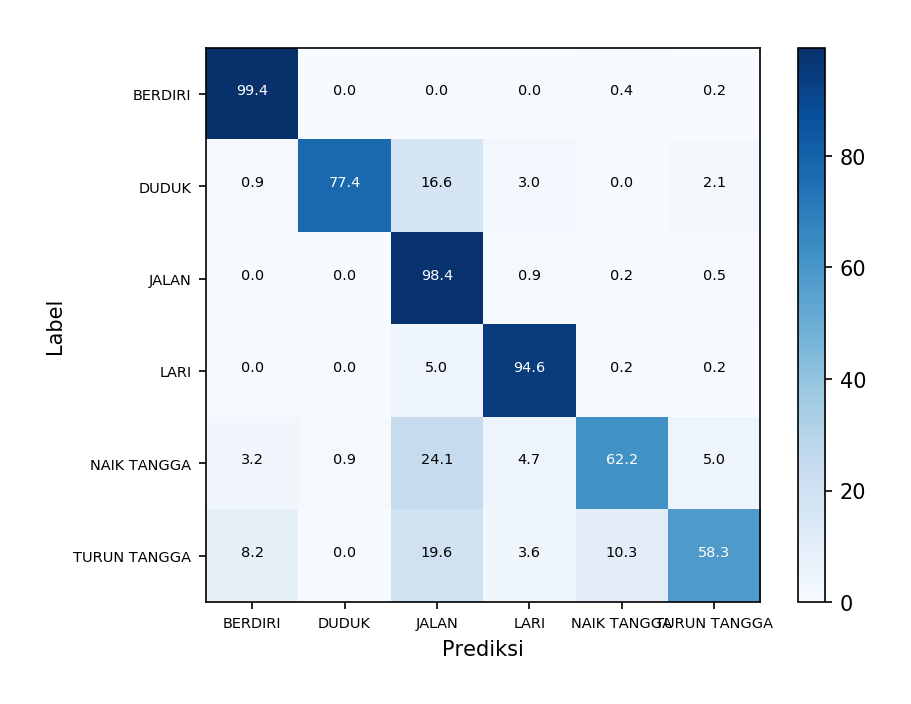
\includegraphics[width=13cm]{gambar/hasil-pembahasan/run34-confusion-matrix.png}
    \caption{\textit{Confusion matrix} pada variasi 28}.
    \label{gambar:run34-confusion-martix}
\end{figure}

Hasil pengujian variasi 8, 17 dan 28 dibandingkan dalam Tabel~\ref{table:perbandingan-model-klasifikasi}. Ketiga variasi tersebut memiliki kelebihan dan kekurangannya masing-masing. Variasi nomor 8 memperoleh akurasi tertinggi pada aktivitas duduk dan lari, namun memperoleh akurasi terendah pada aktivitas berdiri, jalan dan rata-rata akurasi. Variasi nomor 17 memperoleh akurasi tertinggi pada aktivitas naik tangga, turun tangga dan rata-rata akurasi, namun memperoleh akurasi terendah pada aktivitas duduk dan lari. Selain itu variasi nomor 17 juga memiliki arsitektur yang paling sederhana diantara variasi lainnya. Variasi nomor 28 memperoleh akurasi terbaik pada aktivitas berdiri dan jalan, namun memperoleh akurasi terburuk pada aktivitas naik dan turun tangga. Melihat grafik pada Gambar~\ref{gambar:run8-training},~\ref{gambar:run17-training}, dan~\ref{gambar:run34-training}, diketahui bahwa ketiga variasi memiliki penyamarataan yang setara baiknya.

\begin{table}[h!]
    \centering
    \caption{Perbandingan model klasifikasi}
    \begin{threeparttable}
        \begin{tabular}{ |c|c|c|c|c|c|c|c| }
            \hline
            No & B & D & J & L & N & T & Akurasi \\

            \hline
            8 & \cellcolor{red!10} 96,9\% & \cellcolor{teal!20}94,9\% & \cellcolor{red!10} 87,6\% & \cellcolor{teal!20} 96,9\% & 78,6\% & 78,4\% & \cellcolor{red!10} 91,17\% \\

            \hline
            17 & 97,2\% & \cellcolor{red!10} 93,4\% & 96,1\% & \cellcolor{red!10} 85,5\% & \cellcolor{teal!20} 81,2\% & \cellcolor{teal!20} 82,2\% & \cellcolor{teal!20} 93,65\% \\

            \hline
            28 & \cellcolor{teal!20} 99,4\% & 77,4\% & \cellcolor{teal!20} 98,4\% & 94,6\% & \cellcolor{red!10} 62,2\% & \cellcolor{red!10} 58,3\% & 93,15\% \\

            \hline
        \end{tabular}
        \begin{tablenotes}\footnotesize
            \item  B: Berdiri, D: Duduk, J: Berjalan, L: Berlari, N: Naik Tangga, T: Turun Tangga 
        \end{tablenotes}    
    \end{threeparttable}
    \label{table:perbandingan-model-klasifikasi}
\end{table}

Pada ketiga variasi \textit{hyperparameter} tersebut, aktivitas duduk, berdiri, jalan dan lari dapat diklasifikasikan dengan baik karena perbedaan pola yang signifikan pada data-data sensornya, sedangkan aktivitas menaiki tangga dan menuruni tangga memperoleh akurasi yang kurang baik karena pola data sensor yang cukup mirip. Kedua aktivitas tersebut juga memiliki kemiripan dengan aktivitas jalan, sehingga banyak terjadi kesalahan dalam mengklasifikasikan aktivitas menaiki tangga dan menuruni tangga menjadi jalan. Perbandingan pola tersebut dapat dilihat pada Gambar~\ref{gambar:plot-sensor} yang menunjukkan sampel data sensor dari masing-masing aktivitas.

\begin{figure}[h!]
    \begin{subfigure}{0.5\textwidth}
        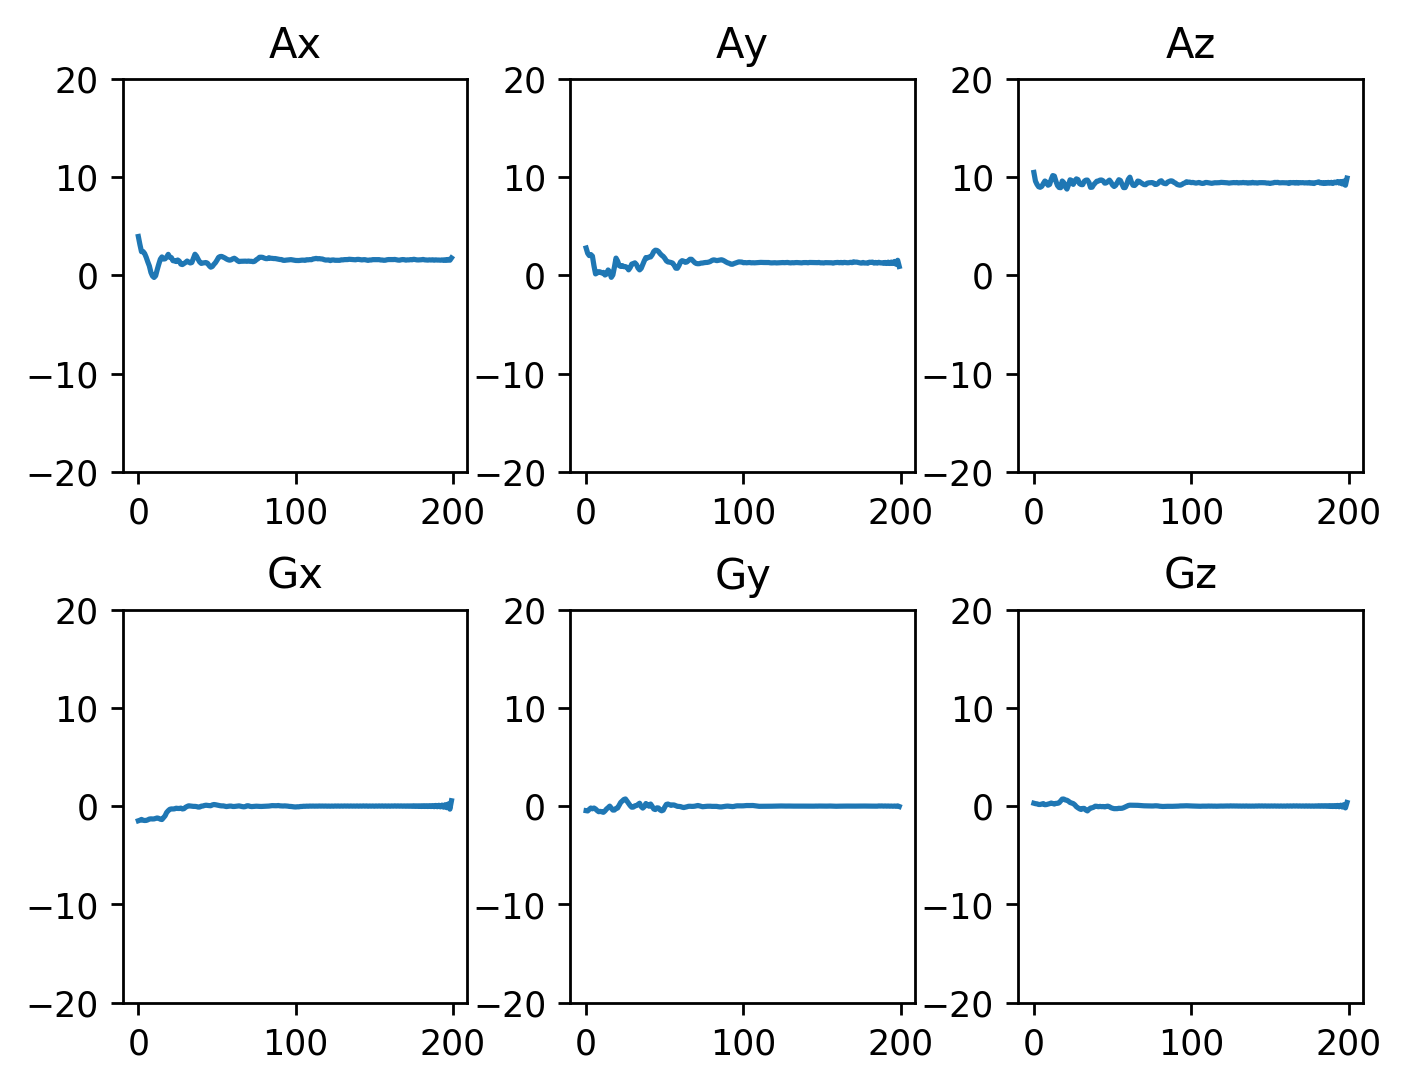
\includegraphics[width=7.2cm]{data/plot-sensor/duduk.png}
        \caption{Duduk}
        \label{gambar:plot-sensor-duduk}
    \end{subfigure}
    \begin{subfigure}{0.5\textwidth}
        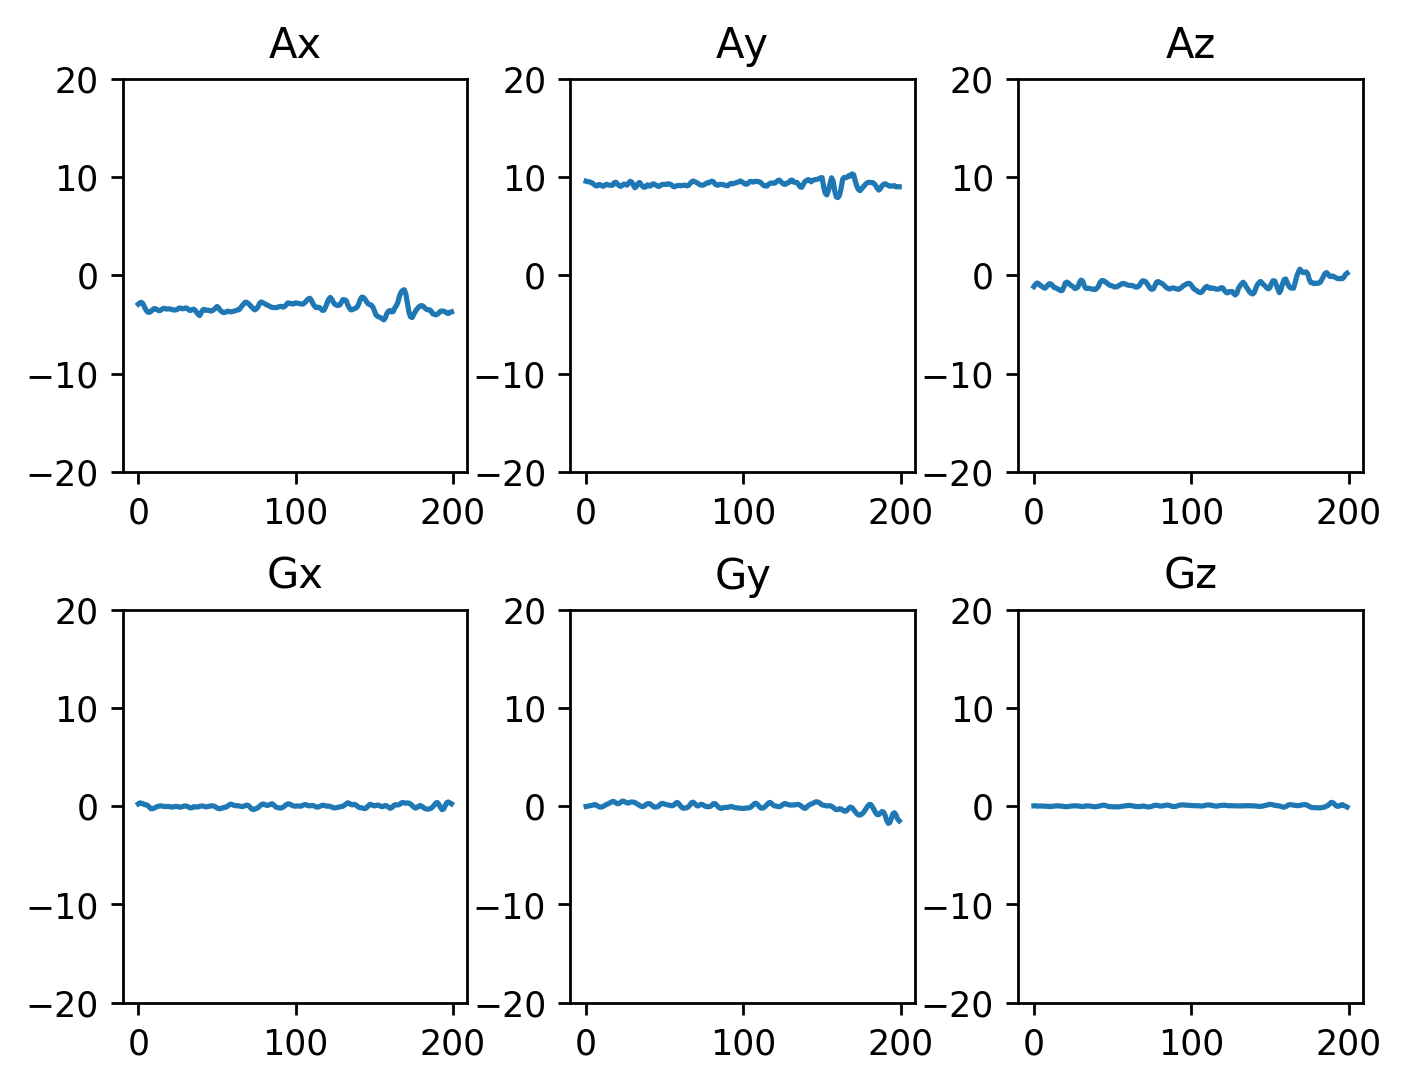
\includegraphics[width=7.2cm]{data/plot-sensor/berdiri.png}
        \caption{Berdiri}
        \label{gambar:plot-sensor-berdiri}
    \end{subfigure}
    \begin{subfigure}{0.5\textwidth}
        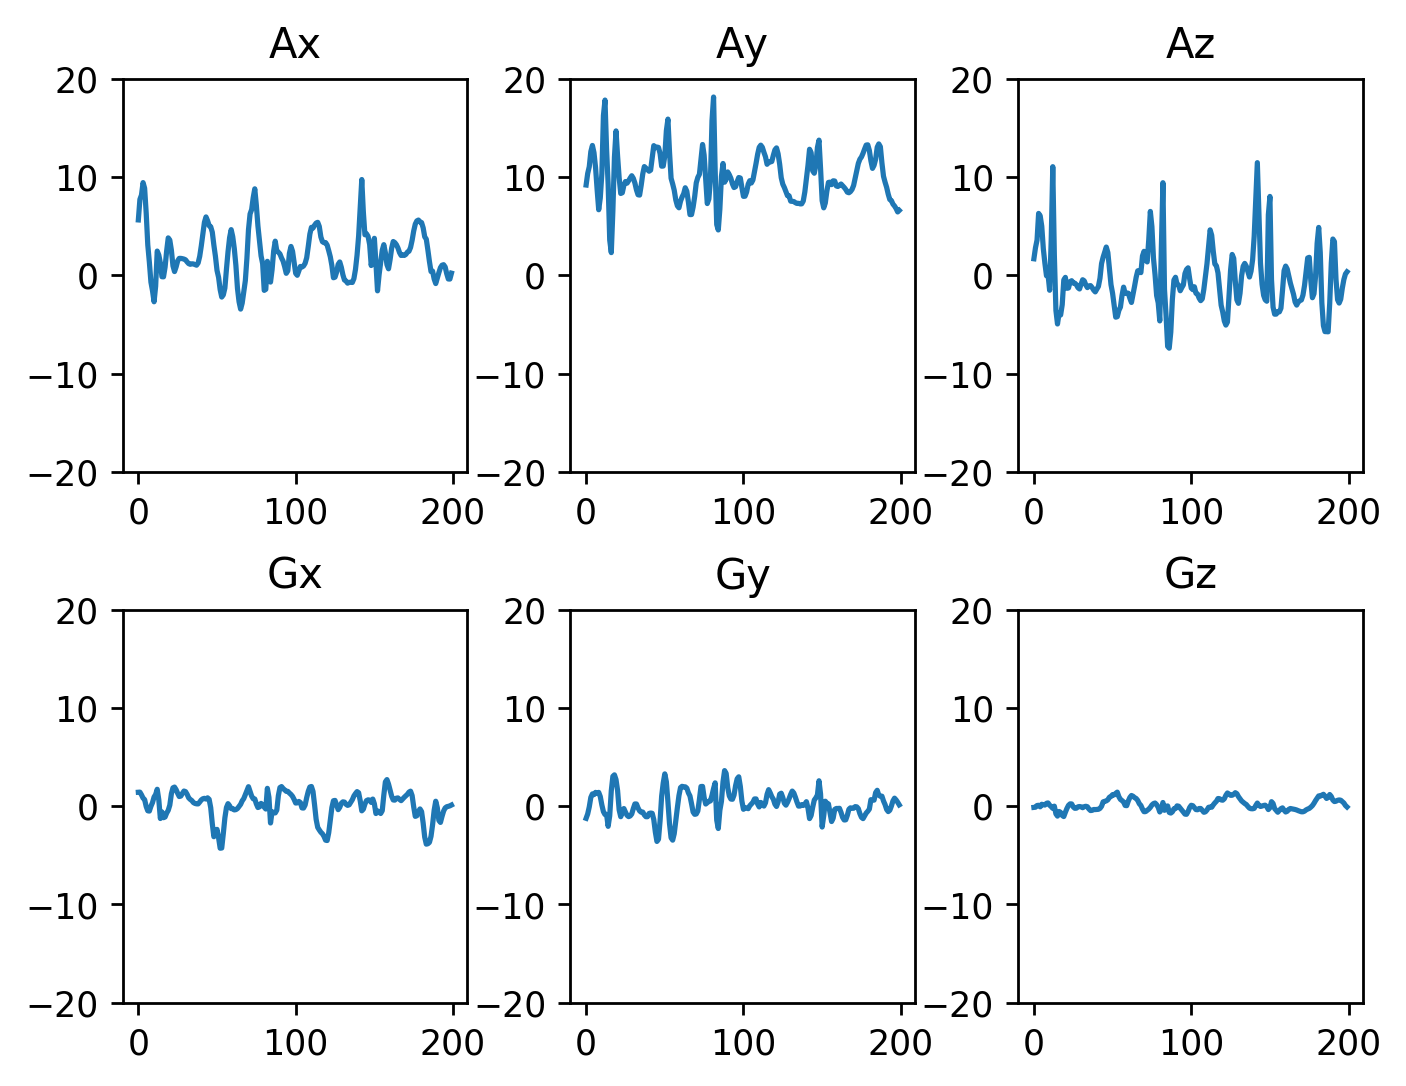
\includegraphics[width=7.2cm]{data/plot-sensor/berjalan.png}
        \caption{Berjalan}
        \label{gambar:plot-sensor-berjalan}
    \end{subfigure}
    \begin{subfigure}{0.5\textwidth}
        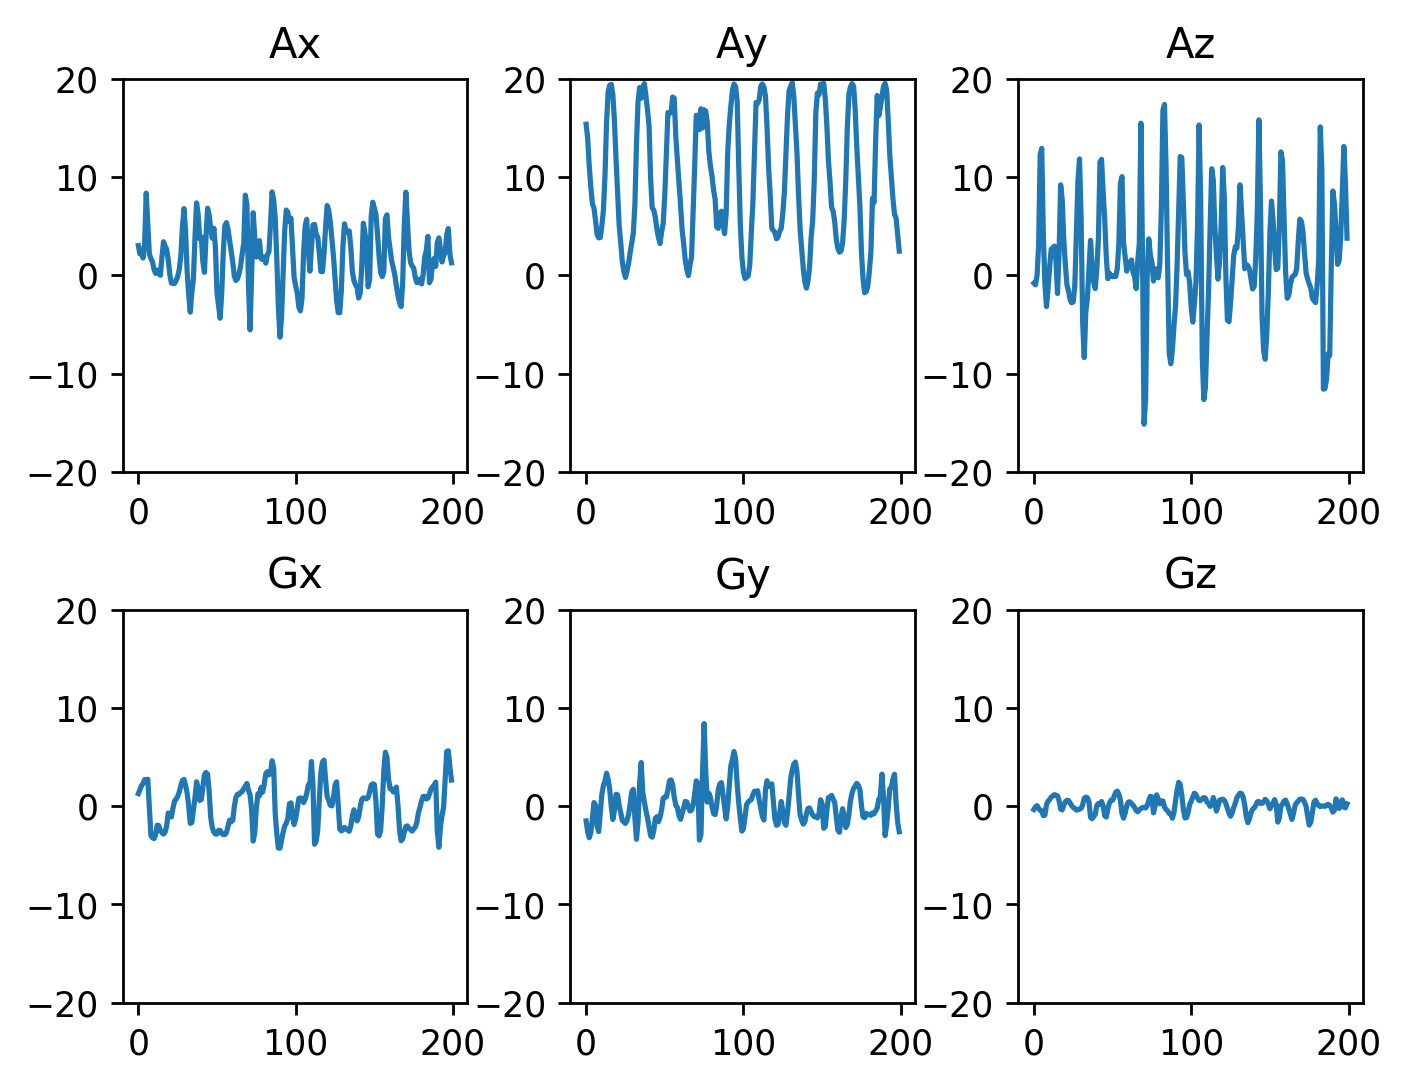
\includegraphics[width=7.2cm]{data/plot-sensor/berlari.png}
        \caption{Berlari}
        \label{gambar:plot-sensor-berlari}
    \end{subfigure}
    \begin{subfigure}{0.5\textwidth}
        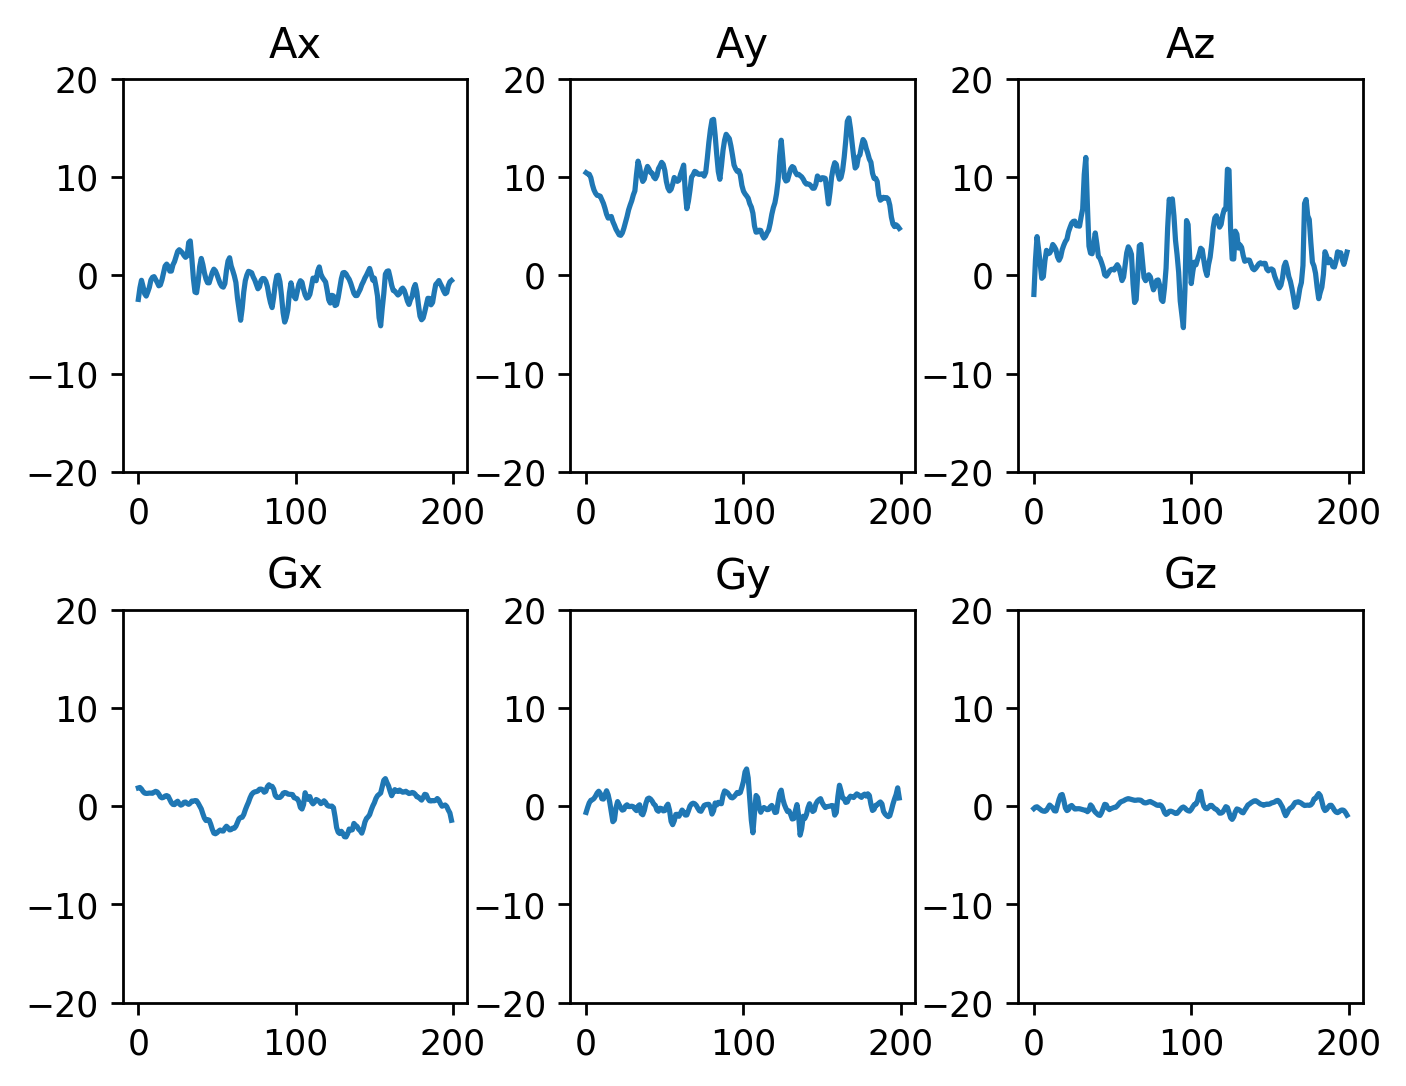
\includegraphics[width=7.2cm]{data/plot-sensor/naik-tangga.png}
        \caption{Menaiki tangga}
        \label{gambar:plot-sensor-naik-tangga}
    \end{subfigure}
    \begin{subfigure}{0.5\textwidth}
        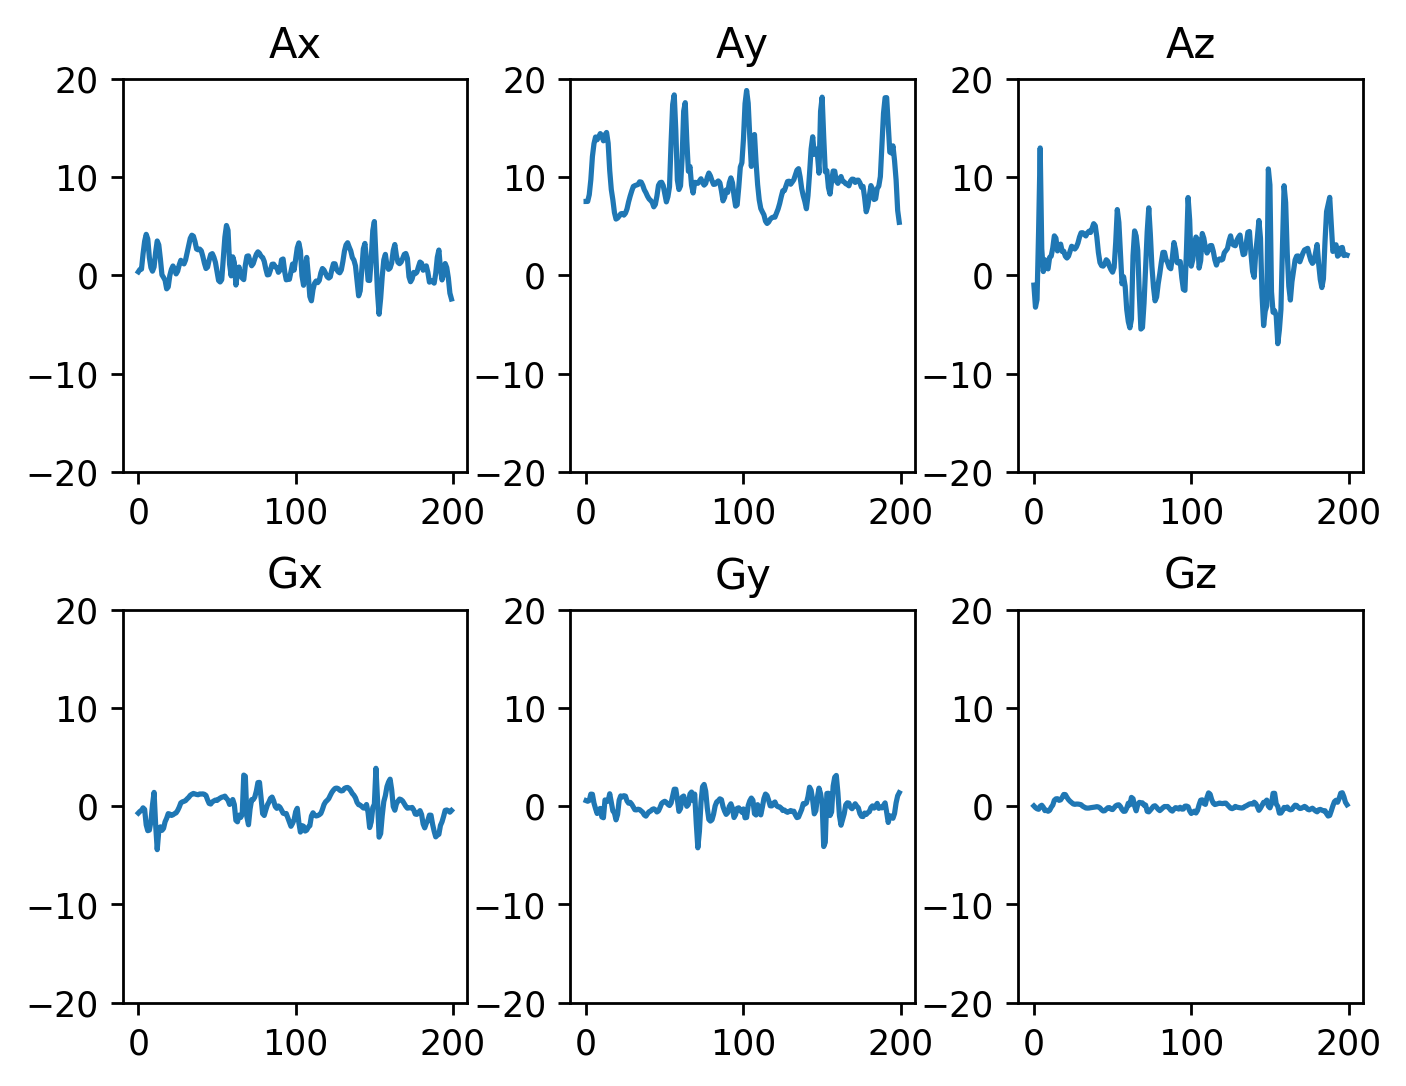
\includegraphics[width=7.2cm]{data/plot-sensor/turun-tangga.png}
        \caption{Menuruni tangga}
        \label{gambar:plot-sensor-turun-tangga}
    \end{subfigure}

    \caption{Perbandingan sinyal sensor dari setiap aktivitas}
    \label{gambar:plot-sensor}
\end{figure}

Berdasarkan pertimbangan kriteria akurasi, penyamarataan dan kompleksitas model, maka variasi nomor 17 dipilih sebagai model terbaik. Model ini kemudian diimplementasikan pada ponsel cerdas pengujian kecepatan klasifikasi.

\section{Hasil Pengujian Kecepatan Klasifikasi pada Ponsel Cerdas}

Pengujian kecepatan klasifikasi pada ponsel cerdas dilakukan untuk mengetahui waktu komputasi yang dibutuhkan model dalam mengklasifikasikan aktivitas pada perangkat dengan kemampuan komputasi yang terbatas. Semakin cepat komputasi dilakukan, maka model dinilai semakin baik digunakan untuk klasifikasi secara \textit{realtime}.

Klasifikasi dilakukan pada tiga ponsel cerdas yang berbeda, yaitu Xiaomi Mi4c dan LG G5 SE, dan vivo V5. Spesifikasi kedua ponsel cerdas tersebut dapat dilihat pada Tabel~\ref{table:spesifikasi-ponsel-cerdas}.

\begin{table}[h!]
    \centering
    \caption{Spesifikasi ponsel cerdas untuk pengujian}
    \begin{tabular}{ |l|l|c|c| }
        \hline
        Ponsel & CPU & Memori & Total Klasifikasi \\

        \hline
        Xiaomi Mi4c & Snapdragon 805 & 2 GB & 887 \\

        \hline
        LG G5 SE & Snapdragon 652 & 3 GB & 413 \\

        \hline
        vivo V5 & Mediatek MT6750 & 4 GB & 332 \\

        \hline
    \end{tabular}
    \label{table:spesifikasi-ponsel-cerdas}
\end{table}

Pengujian dilakukan dengan mencatat waktu komputasi yang diperlukan pada setiap iterasi klasifikasi. Perhitungan waktu dimulai saat jendela data sensor siap digunakan sampai diperoleh prediksi aktivitas. Kecepatan klasifikasi pada ponsel Xiaomi Mi4c diukur oleh tiga partisipan dengan total 887 sampel, kecepatan pada LG G5 SE diukur oleh dua partisipan dengan total 413 sampel, sedangkan kecepatan pada vivo V5 diukur oleh satu partisipan dengan total 332 sampel. Nilai minimum, maksimum, median dan rata-rata diambil dari data yang telah dikumpulkan.

Hasil pengujian dapat dilihat pada Gambar~\ref{gambar:hasil-kecepatan}. Dari 887 klasifikasi yang dilakukan pada ponsel Xiaomi Mi4c, diperoleh waktu komputasi minimal 78 ms, median 148 ms, maksimal 280 ms dan rata-rata 147 ms. Pada ponsel LG G5 SE, dari 413 klasifikasi yang dilakukan, diperoleh waktu komputasi minimal 83 ms, median 176 ms, maksimal 271 ms dan rata-rata 167 ms. Dari 332 klasifikasi yang dilakukan pada ponsel vivo V5, diperoleh waktu komputasi minimal 161 ms, median 229 ms, maksimal 389 ms dan rata-rata 255 ms.

Dari seluruh sampel yang diambil pada ketiga ponsel cerdas, diperoleh waktu komputasi minimal 78 ms, median 174 ms, maksimal 389 ms dan rata-rata 174 ms. Mengingat proses klasifikasi dilakukan setiap minimal satu detik, maka kecepatan tersebut dinilai cukup baik untuk melakukan klasifikasi secara \textit{realtime}.

\begin{figure}[h!]
    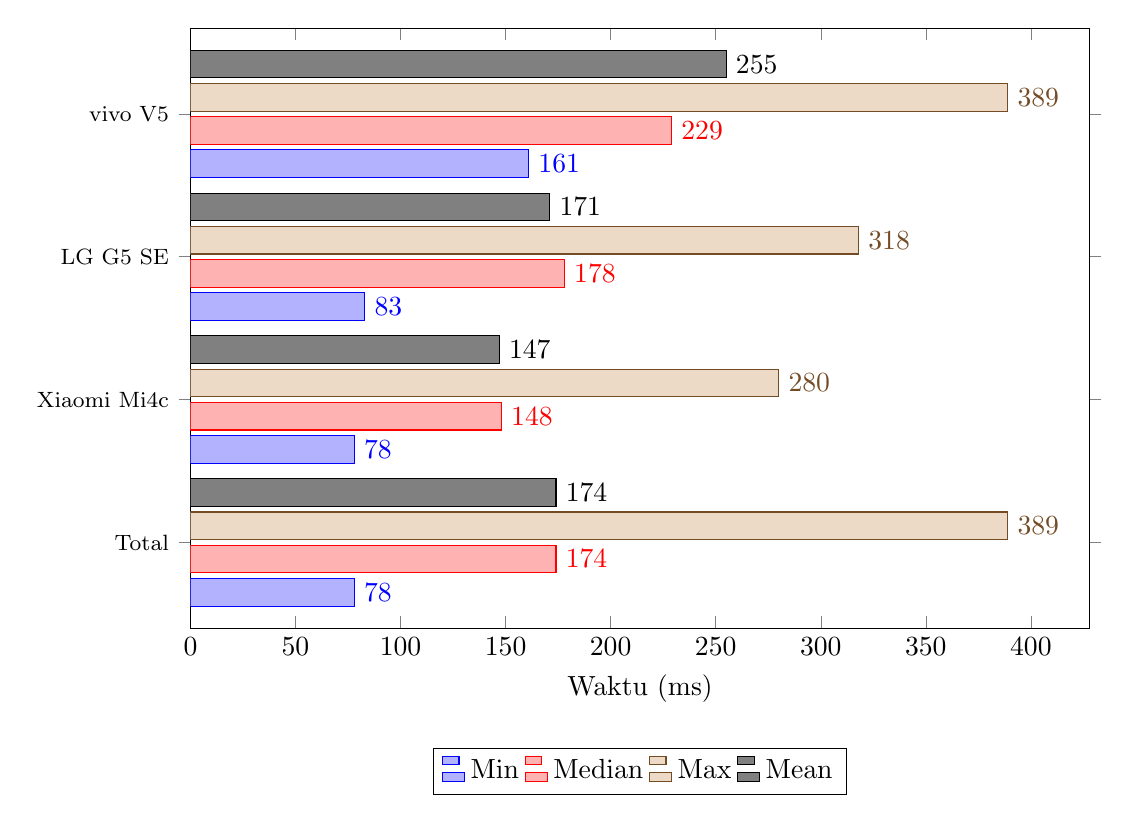
\begin{tikzpicture}
    \begin{axis}[
        xbar, xmin=0,
        y tick label style={font=\footnotesize},
        width=13cm, height=9.2cm, enlarge y limits=0.2,
        xlabel={Waktu (ms)},
        symbolic y coords={Total,Xiaomi Mi4c,LG G5 SE,vivo V5},
        ytick=data,
        nodes near coords, nodes near coords align={horizontal},
        legend style={at={(0.5,-0.20)},
        anchor=north,legend columns=-1},
        ]
        \addplot % Min
        coordinates 
        {(78,Total) (78,Xiaomi Mi4c) (83,LG G5 SE) (161,vivo V5)};
        
        \addplot % Median
        coordinates 
        {(174,Total) (148,Xiaomi Mi4c) (178,LG G5 SE) (229,vivo V5)};
        
        \addplot % Max
        coordinates 
        {(389,Total) (280,Xiaomi Mi4c) (318,LG G5 SE) (389,vivo V5)};

        \addplot % Mean
        coordinates
        {(174,Total) (147,Xiaomi Mi4c) (171,LG G5 SE) (255,vivo V5)};

        \legend{Min,Median,Max,Mean}
    \end{axis}
    \end{tikzpicture}
    \caption{Hasil pengujian kecepatan klasifikasi pada ponsel cerdas}
    \label{gambar:hasil-kecepatan}
\end{figure}

% Perlu dicatat bahwa kecepatan ini hanyalah pendekatan dari waktu komputasi yang sebenarnya. Waktu komputasi diukur dengan ponsel dalam keadaan seperti pada penggunaan sehari-hari, sehingga dipengaruhi oleh beberapa faktor lain seperti penjadwalan sistem operasi dan adanya aplikasi lain yang sedang berjalan di latar belakang.

\chapter{KESIMPULAN DAN SARAN}

\section{Kesimpulan}
Berdasarkan hasil pengujian yang telah dilakukan, telah berhasil dibuat sistem klasifikasi aktivitas manusia menggunakan \textit{Convolutional Neural Network} dan \textit{Long Short-Term Memory} untuk enam aktivitas sederhana, yaitu duduk, berjalan, berdiri, berlari, menaiki tangga dan menuruni tangga dengan akurasi 93,65\%. Pengujian klasifikasi pada tiga ponsel cerdas juga menunjukkan waktu komputasi yang cukup baik untuk melakukan klasifikasi secara \textit{realtime}.

\section{Saran}
Berikut beberapa saran untuk mengembangkan penelitian ini:

\begin{enumerate}
    \item Diperlukan penelitian lebih lanjut untuk meningkatkan akurasi klasifikasi.
    \item Diperlukan penelitian lebih lanjut untuk mengenali aktivitas lainnya.
    \item Diperlukan penelitian lebih lanjut untuk mengurangi \textit{overfitting} pada model.
\end{enumerate}


\setquotestyle{english}
\xpatchbibmacro{date+extrayear}{%
\printtext[parens]%
}{%
\setunit{\addperiod\space}%
\printtext%
}{}{}
\printbibliography[title=DAFTAR PUSTAKA]

\end{document}
